%----------------------------------------------------------------------------------------
%	PACKAGES AND THEMES
%----------------------------------------------------------------------------------------
\PassOptionsToPackage{table}{xcolor}
\documentclass[aspectratio=169,xcolor=dvipsnames,11pt]{beamer}
\usetheme{SimplePlusAIC}
\usepackage{amsmath}
\usepackage{animate}
\usepackage{hyperref}
\usepackage{cleveref}
\usepackage{caption}
\usepackage{graphicx} % Allows including images
\usepackage{subfig}
\usepackage{booktabs} % Allows the use of \toprule, \midrule and  \bottomrule in tables
\usepackage{svg} %allows using svg figures
\usepackage{tikz}
\usepackage{makecell}
\usepackage{multirow}
\usepackage{appendixnumberbeamer}
\usepackage{wrapfig}
\usepackage{verbatim}
\usepackage{tcolorbox}
%\usepackage[dvipsnames]{xcolor}

\usepackage{hhline}
\usepackage{relsize}
\usepackage{bm}
%Select the Epilogue font (requires luaLatex or XeLaTex compilers)
%\setsansfont{Epilogue}[
  %  Path=./epilogueFont/,
  %  Scale=0.9,
  %  Extension = .ttf,
   % UprightFont=*-Regular,
   % BoldFont=*-Bold,
   % ItalicFont=*-Italic,
    %BoldItalicFont=*-BoldItalic
    %]
    \usefonttheme[onlymath]{serif}
% \usepackage{ eulervm } % Euler VM as math serif font

\newcommand*{\defeq}{\stackrel{\text{def}}{=}}
\newcommand{\grad}{\nabla}
\newcommand{\lap}{\Delta}
\newcommand{\weaklyto}{\rightharpoonup}
\newcommand{\weakstar}{\stackrel{*}\rightharpoonup}
\newcommand{\cts}{\hookrightarrow}
\newcommand{\ctsDense}{\xhookrightarrow{d}}
\newcommand{\ctsCompact}{\xhookrightarrow{c}}
\newcommand{\E}{\mathbb{E}}
\newcommand{\pP}{\mathbb{P}}
\newcommand{\R}{\mathbb{R}}
\newcommand{\ER}{\overline{\mathbb{R}}}
\newcommand{\cR}{\mathcal{R}}
\newcommand{\cJ}{\mathcal{J}}
\newcommand{\cG}{\mathcal{G}}
\newcommand{\CVaR}{\textup{CVaR}}
\newcommand{\D}{\textup{ d}}
\newcommand{\dd}{\mathrm{d}}
\newcommand{\fa}{\text{for all }}
\DeclareMathOperator*{\essinf}{\vphantom{p}ess\,inf}
\DeclareMathOperator{\sigmoid}{expit} % a.k.a. logistic sigmoid

\usepackage[ruled,vlined,algo2e]{algorithm2e}
\crefname{algocf}{algorithm}{algorithms}
 \usepackage{caption}

%----------------------------------------------------------------------------------------
%	TITLE PAGE
%----------------------------------------------------------------------------------------

\title[]{The latent variable proximal point algorithm for variational problems with inequality constraints.
 } % The short title appears at the bottom of every slide, the full title is only on the title page
%\subtitle{Subtitle}

\author{\small{\bf Thomas M. Surowiec$^\dagger$}\\  \footnotesize with J. S. Dokken (Simula), P. E. Farrell (Oxford),  B. Keith (Brown U), I.P.A. Papadopoulos (WIAS) }

\institute[\phantom{xxxxxxxxxxxxxxxxxxxxx}]{$^\dagger$Department of Numerical Analysis and Scientific Computing \newline Simula Research Laboratory \newline Oslo, Norway}
% Your institution as it will appear on the bottom of every slide, maybe shorthand to save space


\date{ 
Oxford, 2 April 2025}
%----------------------------------------------------------------------------------------
%	PRESENTATION SLIDES
%----------------------------------------------------------------------------------------

\begin{document}

\begin{frame}[plain]
%\setbeamertemplate{footline}{}
\titlepage
\end{frame}

%\setbeamertemplate{footline}[frame number]

\begin{frame}{Overview}
\tableofcontents
\visible<2->{
{\footnotesize
\begin{thebibliography}{1}

\bibitem{BKeith_TMSurowiec_2024}
{\sc B.~Keith and T.M.~Surowiec.}
\newblock Proximal galerkin: A structure‐preserving finite element method for pointwise bound constraints
\newblock Found. Comut. Math. (2024), \url{https://doi.org/10.1007/s10208-024-09681-8}

\bibitem{JSDokken_etal_2025}
{\sc J.S.~ Dokken, P.E.~Farrell, B.~Keith, I.P.A.~Papadopolous and T.M.~Surowiec.}
\newblock The latent variable proximal point algorithm for variational problems with inequality constraints
\newblock Submitted (2025), \url{https://arxiv.org/abs/2503.05672}
\end{thebibliography}
}
}

\end{frame}

\section{Motivation and Background}
%\begin{frame}\frametitle{Dirichlet's Principle\footnote{\tiny  Due to William Thomson, 1st Lord Kelvin 1847 \& Gau\ss. Named after  Dirichlet by Riemann. Hilbert provided rigorous existence proof in  1900.}}
%
% In contemporary language: for any $f\in L^2(\Omega)$ and $g\in H^1(\Omega)$, the (weak) solution of Poisson's equation over a Lipschitz domain $\Omega \subset \mathbb{R}^n$,
%\begin{equation}
%\label{eq:PoissonEquation}
%	-\Delta u = f
%	\quad \text{in~} \Omega,
%	\qquad
%	u = g \quad \text{on~} \partial\Omega,
%\end{equation}\visible<2->{
%is the \textbf{$H^1(\Omega)$-minimizer} of the Dirichlet energy,
%\begin{equation}
%\label{eq:DirichletEnergy}
%	E(v)
%	=
%	\frac{1}{2}
%	\int_\Omega |\nabla v|^2 \dd x
%	-
%	\int_\Omega v f \dd x
%	\,,
%\end{equation}
%when confined to the \textbf{constraint set} $H^1_g(\Omega) = g + H^1_0(\Omega) = \{ v \in H^1(\Omega) \mid v = g \text{~on~} \partial \Omega\}$.}
%
%\end{frame}

%\begin{frame}\frametitle{A Variational Inequality}
%\begin{itemize}
%\item The  feasible set $H^1_g(\Omega)$ is nonempty, closed, and convex, but not a vector space. 
%\item \visible<2->{
%The Lions--Stampacchia theorem (1967) states that the minimizer $u^\ast \in K = H^1_g(\Omega)$ is the unique solution to a variational inequality (VI)
%\begin{equation*}
%%\label{eq:DirichletVI}
%	\int_\Omega \nabla u^\ast \cdot \nabla (v - u^*)  \dd x \geq \int_\Omega f (v - u^*) \dd x
%	~\fa v \in K.
%	% \int_\Omega (\nabla v - \nabla u) \cdot \nabla u \dd x \geq \int_\Omega (v-u) f \dd x
%	% ~\fa v \in K.
%\end{equation*}
%}
%\end{itemize}
%\visible<3->{
%\begin{center}\textit{
%But no one solves Poisson's problem \eqref{eq:PoissonEquation} as a variational inequality. Why not?}
%\end{center}
%}
%\end{frame}

%\begin{frame}\frametitle{Back to the Dirichlet's Principle}
%\begin{itemize}
%\item $K = H^1_g(\Omega)$ is affine and for all $w \in H^1_0(\Omega)$ and $v \in H^1_g(\Omega)$, $v + w \in H^1_g(\Omega)$, as well. \pause
%\item Taking $v = u^\ast\pm w$ for any $w \in H^1_0(\Omega)$ here
%\begin{equation*}
%	\int_\Omega \nabla u^\ast \cdot \nabla (v-u^*)  \dd x \geq \int_\Omega f (v - u^*) \dd x
%	~\fa v \in K,
%	% \int_\Omega (\nabla v - \nabla u) \cdot \nabla u \dd x \geq \int_\Omega (v-u) f \dd x
%	% ~\fa v \in K.
%\end{equation*}
%brings us back to Dirichlet's principle: Find $u^* \in H^1_g(\Omega)$ such that
%\begin{equation*}
%	\int_\Omega \nabla u^\ast \cdot \nabla w \dd x = \int_\Omega f w \dd x
%	~\fa w \in H^1_0(\Omega).
%\end{equation*}
%\end{itemize}\pause
%\begin{center}\textit{
% We use the explicit \textit{geometry} of the feasible set to derive a simpler problem.
% }
% \end{center}
%\end{frame}

%\begin{frame}\frametitle{The Obstacle Problem\footnote{\tiny Introduced by G.\ Stampacchia around 1963. Variational inequalities proposed by A. Signorini (1959) and studied by G. Fichera (1963) and onwards.}}
%%\begin{itemize}
%%\item 
%We seek an  \textbf{$H^1(\Omega)$-minimizer} $u$ of the Dirichlet energy:
%\begin{equation*}
%%\label{eq:DirichletEnergy}
%	E(v)
%	=
%	\frac{1}{2}
%	\int_\Omega |\nabla v|^2 \dd x
%	-
%	\int_\Omega v f \dd x
%	\,,
%\end{equation*}
%over the \textbf{closed convex cone} defined by  
%\[
%K = \{ v \in H^1_0(\Omega) \mid v \geq 0 \text{~a.e.}\}% = H^1_0(\Omega) \cap H^1_+(\Omega).
%\] 
%%\item 
%\visible<2->{This can be reformulated as a \textbf{variational inequality}:
%\begin{equation*}%\label{eq:obs_vi}
%       \text{Find } u \in K : 
%	\int_\Omega \nabla u \cdot \nabla (v-u)  \dd x \geq \int_\Omega f (v - u) \dd x
%	~\fa v \in K.
%	% \int_\Omega (\nabla v - \nabla u) \cdot \nabla u \dd x \geq \int_\Omega (v-u) f \dd x
%	% ~\fa v \in K.
%\end{equation*}
%}
%%\vspace{-2ex}
%%\item 
%\visible<3->{This cannot be rewritten as \textbf{variational equation}.}\vspace{1ex}
%%\end{itemize}
%\end{frame}

\begin{frame}\frametitle{The Obstacle Problem\footnote{\tiny Introduced by G.\ Stampacchia around 1963. Variational inequalities proposed by A. Signorini (1959) and studied by G. Fichera (1963) and onwards.}}
\visible<2->{
  \begin{minipage}{0.48\textwidth}
  \begin{beamercolorbox}[rounded=true, shadow=true, wd=\textwidth]{block title}
We seek an  \textbf{$H^1(\Omega)$-minimizer} $u$ of the Dirichlet energy:
\begin{equation*}
	E(v)
	=
	\frac{1}{2}
	\int_\Omega |\nabla v|^2 \dd x
	-
	\int_\Omega v f \dd x
	\,,
\end{equation*}
over the \textbf{closed convex cone} defined by  
\[
K = \{ v \in H^1_0(\Omega) \mid v \geq 0 \text{~a.e.}\}
\] 
   \end{beamercolorbox}
    \end{minipage}}
    \hfill
     \visible<3->{
    \begin{minipage}{0.48\textwidth}
      \begin{beamercolorbox}[rounded=true, shadow=true, wd=\textwidth]{block title}
       This yields a \textbf{variational inequality}:\\ Find $u \in K$:
	\begin{equation*}
	\int_\Omega \nabla u \cdot \nabla (v-u)  \dd x \geq \int_\Omega f (v - u) \dd x
	\end{equation*}
	$\fa v \in K$.\medskip
	
\visible<4->{We cannot write this as \textbf{variational equation}.}
\end{beamercolorbox}
\end{minipage}}
\end{frame}


\section{Algorithms and First Numerical Experiments}
\begin{frame}\frametitle{Solving Variational Inequalities}
\begin{itemize}
\item \visible<1->{Many possibilities: penalty methods, interior point methods, augmented Lagrangian.}
\item \visible<2->{The obstacle problem can be viewed as a \textit{mixed complementarity problem}:\\ Find $(u,\lambda) \in H^1_0(\Omega) \times H^{-1}(\Omega)$ s.t.
\[
\underbrace{-\Delta u - \lambda = f,}_{\text{PDE}} \quad \underbrace{u \ge 0 \quad {\color{red}``\lambda \ge 0"}, \quad \langle \lambda, u \rangle = 0}_{\text{Complementarity Condition}}.
\]}
\end{itemize}
\begin{minipage}{0.5\linewidth}
\begin{itemize}
\item \visible<3->{
$\lambda$ has low regularity. 
\item This results in \textit{mesh dependence}\footnote{\tiny The number of iterations needed to reach the same stopping tolerance increases with mesh refinements.}  for methods tacitly requiring $\lambda \in L^2(\Omega)$.
}
\item \visible<4->{$\text{Leb}(\left\{x \in \Omega : u(x) = 0,\; \lambda(x) = 0 \right\}) > 0$ causes numerical instabilities.
\item ``Loss of strict complementarity''
}
\end{itemize}
\end{minipage}\qquad
\begin{minipage}{0.4\linewidth}
\centering\visible<3->{
	\begin{tikzpicture}
		\node at (-1.35,1.25) {\includegraphics[clip=true, trim= 4cm 0 0 0, height=4cm]{Figures/ObstacleExperiment2.png}};
		% \node at (-3.35,1) {\includegraphics[clip=true, trim= 4cm 0 0 0, width=0.44\textwidth]{Figures/ObstacleExperiment2.png}};
%		\node at (3,0.4) {
%		   \includegraphics[clip=true, trim= 0 0 0.35cm 0, height=2.1in]{Figures/tikz/FEniCS_plots/example1/example1_ConvergenceRate.pdf}
%		};
	    % \node at (-4,2.8) {\includegraphics[height=2cm]{Figures/tikz/FEniCS_plots/example1/colorbar/colorbar1.pdf}};
	    \node at (-3.7,0.5) {\includegraphics[height=2cm]{Figures/tikz/FEniCS_plots/example1/colorbar/colorbar1.pdf}};
	    \node at (0.75,2.2) {\includegraphics[height=2cm]{Figures/tikz/FEniCS_plots/example1/colorbar/colorbar2.pdf}};
    \end{tikzpicture}
}
\end{minipage}
\end{frame}

\begin{frame}\frametitle{Solving Variational Inequalities}
\begin{itemize}
\item An idea from convex optimization: the proximal point method.\footnote{\tiny Introduced by B. Martinet (1970). Based on a proof idea in Lions \& Stampacchia (1967). See also Bregman (1967), Nemirovsky \& Yudin (1983)}
\item \visible<2->{Given $\alpha > 0$ and previous iterate $v$, find $u^{*} \in K$ that minimizes 
\[
\underbrace{E(u)}_{\text{Objective}} + \underbrace{\frac{1}{\alpha} \int_{\Omega} u \ln\left(\frac{u}{v}\right) - (u + v) \, \mathrm{d}x}_{\text{Bregman distance induced by Shannon entropy}} \text{ over } K. 
\]
}\vspace{-2ex}
\item \visible<3->{The optimality conditions for this problem (after a rather fine analysis) become 
\begin{equation}\label{eq:primal-entro-poisson}
	\begin{aligned}
					\,-\Delta u + \only<3>{{\color{Black}\alpha^{-1}\ln u}}\only<4->{\alert{\alpha^{-1}\ln u}}
					&=
					f + \alpha^{-1}\ln w
					~~ &&\text{in~} \Omega\,,
					\\
					u
					&=
					g ~~ &&\text{on~} \partial\Omega\,.
				\end{aligned}
				\end{equation}
				}\vspace{-3ex}
\item \visible<4->{
But solving \eqref{eq:primal-entro-poisson} as is with Newton's method \alert{does not work very well.}
}
\end{itemize}
\end{frame}



%\begin{frame}\frametitle{A Meta-Algorithm}
%\begin{algorithm2e}[H]
%\DontPrintSemicolon
%	\caption{\label{alg:HomogeneousAlg} Entropic proximal point algorithm for an obstacle problem.}
%	\SetKwInOut{Input}{input}
%	\BlankLine
%	\Input{Step size parameter $\alpha>0$ and initial solution guess $w \in H^1_g(\Omega)\cap L^\infty(\Omega)$ s.t.\ $\essinf w > 0$.
%	 $f \in L^\infty(\Omega)$ and $g_{|\partial\Omega} \in C(\partial \Omega)$ s.t.\ $\essinf_{\partial\Omega} g > 0$.}
%	\BlankLine
%	\Repeat{a convergence test is satisfied}
%	{
%		Solve the \textit{entropic Poisson equation},
%		\begin{equation}
%		\label{eq:EPEIntro}
%			\left\{
%				\begin{aligned}
%					\,-\Delta u + {\color{Red}\alpha^{-1}\ln u}
%					&=
%					f + \alpha^{-1}\ln w
%					~~ &&\text{in~} \Omega\,,
%					\\
%					u
%					&=
%					g ~~ &&\text{on~} \partial\Omega\,.
%				\end{aligned}
%			\right.
%		\end{equation}
%		\;
%		\vspace*{-\baselineskip}
%		Assign $w \leftarrow u$.\;
%	}
%	\BlankLine
%\end{algorithm2e}
%
%\end{frame}



\begin{frame}\frametitle{Entropic Poisson $\rightarrow$ Saddle Point}
\begin{itemize}
\item
Introduce \textbf{latent variables} $\psi, \widetilde{\psi} \in W$ (latent space) : $u = \exp(\psi)$ and $\widetilde{\psi} = \ln w$ 
\item \visible<2->{Transforms \eqref{eq:primal-entro-poisson} into a nonlinear saddle point problem in $(u,\psi)$:
\begin{equation}\label{eq:lvpp-spp-obstacle}
	\begin{aligned}
					\,-\alpha \Delta u + \alert{\psi}
					&=
					\alpha f + \alert{\widetilde{\psi}}
					~~ &&\text{in~} \Omega\,,
					\\
					\alert{u
					-
					\exp(\psi)}
					&=
					0
					~~ &&\text{in~} \Omega\,,
					\\
					u
					&=
					g ~~ &&\text{on~} \partial\Omega\,.
				\end{aligned}
				\end{equation}
%		\begin{gather*}
%			\left\{
%			\begin{aligned}
%				\,&\text{Find}~
%				u\in H^1_g(\Omega) ~\text{and}~\psi \in W
%				~\text{such that~}
%				\\
%				&\begin{alignedat}{4}
%					\int_\Omega \alpha \nabla u\cdot \nabla v \dd x + \int_\Omega \psi v \dd x &= \int_\Omega (\alpha f + \widetilde{\psi})\, v \dd x
%					&&~\fa v \in H^1_0(\Omega)
%					\,,
%					\\
%					\int_\Omega u \varphi \dd x - \int_\Omega \exp(\psi) \varphi \dd x &= 0
%					&&~\fa \varphi \in W
%					\,.
%				\end{alignedat}
%			\end{aligned}
%			\right.
%		\end{gather*} 
		}
\end{itemize}
\visible<3->{
\begin{center}
\textit{
Regardless of the choice or order of approximating spaces for $H^1_g(\Omega)$ and $W$ the discrete solution $\psi_h$ yields a \textbf{latent solution} $\widetilde{u}_h := \exp(\psi_h)$ 
that is \alert{globally bound preserving on the discrete level}.
}
\end{center}}
%\visible<4->{
%\begin{itemize}
%\item $V_h \subset H^1(\Omega)$, $W_h \subset L^1(\Omega)$ are finite dimensional subspaces with parameter $h > 0$.
%\end{itemize}
%}
\end{frame}

\begin{frame}\frametitle{Proximal Galerkin}{\small
\begin{algorithm2e}[H]
\DontPrintSemicolon
	\caption{\label{alg:EntropicGalerkinIntro} 	Discrete saddle point subproblems}
%	\SetKwInOut{Input}{Input}
%	\SetKwInOut{Output}{Output}
%	\BlankLine
%	\Input{Step size $\alpha > 0$, subspaces $V_h \subset H^1_0(\Omega)$ and $W_h \subset L^\infty(\Omega)$, and initial guess $\psi_h \in W_h$.}
%	\Output{Approximate solutions $u_{h}$ and $\widetilde{u}_h = \exp\psi_h$, and approximate Lagrange multiplier, $\lambda_h = (\omega_h - \psi_h)/\alpha$.}
%	% \Output{Two approximate solutions, $u_{h}$ and $\widetilde{u}_h = \exp(\alpha\psi_h)$, and an approximate Lagrange multiplier, $\lambda_h = \omega_h - \psi_h$.}
%	\BlankLine
	\Repeat{a convergence test is satisfied}
	{
		Assign $\omega_h \leftarrow \psi_{h}$ and solve (using e.g. Newton's method):
%		solve the following (nonlinear) discrete saddle-point problem:  
		\vspace{-2ex}
		\begin{gather*}
		% \label{eq:ObstacleDiscreteNonlinearSaddlePoint}
			\left\{
			\begin{aligned}
				\,&\text{Find}~
				u_{h}\in g_h + V_{h} ~\text{and}~\psi_{h} \in W_{h}
				% u_{h}\in V_{h} + g_{h} ~\text{and}~\psi_{h} \in W_{h}
				~\text{such that~}
				\\
				&\begin{alignedat}{4}
					\int_\Omega \alpha \nabla u_h\cdot \nabla v \dd x + \int_\Omega \psi_h v \dd x &= \int_\Omega (\alpha f + \omega_h)\, v \dd x
					&&~\fa v \in V_h
					\,,
					\\
					\int_\Omega u_h \varphi \dd x - \int_\Omega \exp(\psi_h) \varphi \dd x &= 0
					&&~\fa \varphi \in W_h 
					\,.
				\end{alignedat}
			\end{aligned}
			\right.
		\end{gather*}
		\;
		\vspace*{-\baselineskip} \vspace{-2ex}
	}
\end{algorithm2e}
}
{\small
\begin{itemize}
\item The \alert{full algorithm} requires updating $\alpha$, $\omega$ and repeating \Cref{alg:EntropicGalerkinIntro}.
\item $\alpha > 0$ \alert{can remain fixed} or updated successively provided  $\sum \alpha = \infty$.
\item \alert{Convergence} given by the  proximal point method with \alert{rate} $O((\sum \alpha)^{-1/2})$.
\item The rate \alert{is independent of $h$} and holds on the continuous level. 
\end{itemize}
}
\end{frame}

%\begin{frame}\frametitle{}
%\thispagestyle{empty}
%\begin{center}
%{\Large 
%{\color{Maroon}
%But does it actually work?
%}
%}
%\end{center}
%\end{frame}

%\begin{frame}\frametitle{A Word about Theory}
%\begin{itemize}
%\item We will see later that the underlying method arises from the discretization of a special class singularly perturbed nonlinear saddle point problems.
%\item Rigorous, but technical, theory for the obstacle problem in Sec. 5 of the manuscript!
%\item Requires working in $H^1_{g}(\Omega) \cap L^{\infty}(\Omega)$.
%\end{itemize}
%\end{frame}

%\begin{frame}\frametitle{Finite Element Spaces}
%\begin{itemize}
%\item In order to get a stable pair of FE spaces, we suggest a particular pairing.
%\item We refer to the following as the $(\mathbb{P}_p\text{-bubble},\mathbb{P}_{p-1}\text{-broken})$ pairing:
%\begin{equation*}
%\label{eq:SubspacePair1}
%	V_h = \mathbb{P}_{p}^{p+2}(\mathcal{T}_h)\cap H^1_0(\Omega)
%	\,,\qquad
%	% \quad
%	% \text{and}
%	% \quad
%	W_h = \mathbb{P}_{p-1}(\mathcal{T}_h)
%	\,.
%\end{equation*}
%\item $V_h$ comprises globally continuous functions that are direct sums of $(p+2)$-order bubble functions and $p$-order polynomials (on the cells).
%\item $W_h$ is generated by bounded functions that $(p-1)$-polynomials (on the cells).
%\item E.g., $p = 1$: $V_h$ is composed of the direct sum of piecewise linear functions and 3rd order bubble functions and $W_h$ is piecewise constants.
%\end{itemize}
%\end{frame}


\begin{frame}\frametitle{Experiment 1}
\begin{center}
{\color{Maroon} \Large How does PG behave over various meshes and polynomials orders?}
\end{center}
\end{frame}

\begin{frame}\frametitle{Experiment 1}
\begin{itemize}
\item $\Omega := \Omega_{\infty} = [-1,1]\times[-1,1] \subset \mathbb R^2$.
\item Set $g=u$, where $u(x,y)$ is the smooth manufactured solution
\begin{equation}
\label{eq:Biactivity_SmoothManufacturedSolution}
	u(x,y)
	=
	\begin{cases}
		0 & \text{if~} x < 0\,,\\
		x^4 & \text{otherwise,}\\
	\end{cases}
	\quad
	% \iff
	\text{implied by}
	% \impliedby
	\quad
	f(x,y)
	=
	\begin{cases}
		0 & \text{if~} x < 0\,,\\
		-12x^2 & \text{otherwise.}\\
	\end{cases}
\end{equation}
\item \visible<2->{$\lambda \equiv 0$: \alert{strict complementarity fails} on large subset of $\Omega$!}
%\item The active/contact set has positive Lebesgue measure.
\item \visible<3->{Proximal point is a (slow) fixed point method if $\alpha$ is left fixed. 
\item We choose $\left\{\alpha_k\right\}$ with $\alpha_1 = 1$ and $\alpha_k$ \alert{increasing} to a maximum value of $10^{10}$. 
%: 
%\begin{equation}
%\label{eq:ObstacleStepSizes_superexponential}
%	\alpha_1 = 1\,,
%	\quad
%	\alpha_k
%	=
%	\min\bigl\{ \max\bigl\{\alpha_1,r^{q^{k-1}} - \alpha_{k-1}\bigr\} , 10^{10} \bigr\}
%	\,,
%	\quad
%	k = 2,3,\ldots,
%\end{equation}
%where $r = q = 1.5$. 
} 
%\item \visible<4->{
%Once $\alpha_k = 10^{10}$, we can check successive iterates as a stopping criterion.
%}
\end{itemize}
\end{frame}

\begin{frame}\frametitle{Experiment 1: Results}
\begin{figure}
	\centering
	\begin{tikzpicture}
		\node at (-3.35,0.5) {\includegraphics[height=1.5in]{Figures/ObstacleExperiment1.png}};
		\node at (3.25,0.4) {
			   \includegraphics[clip=true, trim= 0 0 0.35cm 0, height=2.1in]{Figures/tikz/FEniCS_plots/example0/example0_ConvergenceRate.pdf}
		};
	    \node at (-0.5,0.4) {\includegraphics[height=2cm]{Figures/tikz/FEniCS_plots/example0/colorbar/colorbar0.pdf}};
	    \node at (-2.2,-1.35) {\scriptsize $
	    	u(x,y)
	    	=
	    	\begin{cases}
	    		0 & \text{if~} x < 0\\
	    		x^4 & \text{otherwise}\\
	    	\end{cases}
	    $};
    \end{tikzpicture}
%	\caption{
%	\label{fig:BiactiveIterationComplexity}
%	Biactivity.
%	Verifying the convergence orders predicted by \Cref{cor:ConvergenceRates} with the $(\mathbb{P}_1\text{-bubble},\mathbb{P}_{0}\text{-broken})$ discretization (FEniCSx).
%	Left: The exact solution.
%	Right: Plots of the optimization error $\|u_h - u_h^k\|_{H^1(\Omega_\infty)}$ and corresponding step size $\alpha_k$ when $h = h_\infty / 16$.
%	The blue curve tracks the \emph{sublinear} convergence induced by the fixed step size rule $\alpha_k = 1$.
%	Meanwhile, the step size rules \cref{eq:ObstacleStepSizes_geometric} and \cref{eq:ObstacleStepSizes_superexponential} induce \emph{linear} (red) and \emph{superlinear} (green) convergence, respectively.
%	The results are similar on finer meshes due to mesh-independence; cf.~\Cref{tab:BiactivityMeshIndependence}.
%	}
\end{figure}
\hypertarget{example_1}{}
 \hyperlink{target}{\beamerbutton{Go to Finite Element Spaces}}
\end{frame}

\begin{frame}\frametitle{Experiment 1: Results}

\begin{table}
\centering
\tiny
\renewcommand{\arraystretch}{1.3}
\begin{tabular}{ |c|c|c|c|c|c|c| }
 \hhline{|>{\arrayrulecolor{white}}-->{\arrayrulecolor{black}}|-----|}
 \multicolumn{2}{c|}{} & \multicolumn{5}{c|}{\cellcolor{lightgray!15} \small\raisebox{5pt}{\vphantom{f}} Progress of the iterates $\|u_h^{k} - u_h^{k-1}\|_{H^1(\Omega_\infty)}$ for various $h$ and $p$}\\[3pt]
 \hhline{|>{\arrayrulecolor{white}}-->{\arrayrulecolor{black}}|-----|}
 \multicolumn{2}{c|}{}& \multicolumn{3}{c|}{\cellcolor{lightgray!05} Polynomial order $p = 1$} & \multicolumn{2}{c|}{\cellcolor{lightgray!10} Polynomial order $p = 2$}\\
 \hline
 \rowcolor{lightgray!15}
 $k$ & $\alpha_{k}$ & $h_\infty/16$ & $h_\infty/32$ & $h_\infty/64$ & $h_\infty/16$ & $h_\infty/32$ \\
 \hline
\cellcolor{lightgray!05}   1 & \cellcolor{lightgray!01}   $1.0$              & $2.10\cdot 10^{0}$   & $2.10\cdot 10^{0}$   & $2.10\cdot 10^{0}$   & $2.10\cdot 10^{0}$   & $2.10\cdot 10^{0}$   \\
\cellcolor{lightgray!05}   2 & \cellcolor{lightgray!01}   $1.0$              & $6.45\cdot 10^{-1}$  & $6.45\cdot 10^{-1}$  & $6.45\cdot 10^{-1}$  & $6.45\cdot 10^{-1}$  & $6.45\cdot 10^{-1}$  \\
\cellcolor{lightgray!05}   3 & \cellcolor{lightgray!01}   $1.49$             & $1.73\cdot 10^{-1}$  & $1.73\cdot 10^{-1}$  & $1.73\cdot 10^{-1}$  & $1.73\cdot 10^{-1}$  & $1.73\cdot 10^{-1}$  \\
\cellcolor{lightgray!05}   4 & \cellcolor{lightgray!01}   $2.43$             & $1.10\cdot 10^{-1}$  & $1.10\cdot 10^{-1}$  & $1.10\cdot 10^{-1}$  & $1.10\cdot 10^{-1}$  & $1.10\cdot 10^{-1}$  \\
\cellcolor{lightgray!05}   5 & \cellcolor{lightgray!01}   $5.35$             & $7.76\cdot 10^{-2}$  & $7.77\cdot 10^{-2}$  & $7.77\cdot 10^{-2}$  & $7.77\cdot 10^{-2}$  & $7.77\cdot 10^{-2}$  \\
\cellcolor{lightgray!05}   6 & \cellcolor{lightgray!01}   $1.64\cdot 10^{1}$ & $4.76\cdot 10^{-2}$  & $4.77\cdot 10^{-2}$  & $4.77\cdot 10^{-2}$  & $4.77\cdot 10^{-2}$  & $4.77\cdot 10^{-2}$  \\
\cellcolor{lightgray!05}   7 & \cellcolor{lightgray!01}   $8.50\cdot 10^{1}$ & $2.24\cdot 10^{-2}$  & $2.25\cdot 10^{-2}$  & $2.25\cdot 10^{-2}$  & $2.25\cdot 10^{-2}$  & $2.25\cdot 10^{-2}$  \\
\cellcolor{lightgray!05}   8 & \cellcolor{lightgray!01}   $9.35\cdot 10^{2}$ & $5.82\cdot 10^{-3}$  & $5.84\cdot 10^{-3}$  & $5.85\cdot 10^{-3}$  & $5.85\cdot 10^{-3}$  & $5.85\cdot 10^{-3}$  \\
\cellcolor{lightgray!05}   9 & \cellcolor{lightgray!01}   $3.17\cdot 10^{4}$ & $6.04\cdot 10^{-4}$  & $6.07\cdot 10^{-4}$  & $6.07\cdot 10^{-4}$  & $6.07\cdot 10^{-4}$  & $6.07\cdot 10^{-4}$  \\
\cellcolor{lightgray!05}  10 & \cellcolor{lightgray!01}   $5.85\cdot 10^{6}$ & $1.80\cdot 10^{-5}$  & $1.81\cdot 10^{-5}$  & $1.81\cdot 10^{-5}$  & $1.81\cdot 10^{-5}$  & $1.81\cdot 10^{-5}$  \\
\cellcolor{lightgray!05}  11 & \cellcolor{lightgray!01}   $1\cdot 10^{10}$   & $9.41\cdot 10^{-8}$  & $9.47\cdot 10^{-8}$  & $9.49\cdot 10^{-8}$  & $9.50\cdot 10^{-8}$  & $9.50\cdot 10^{-8}$  \\
\cellcolor{lightgray!05}  12 & \cellcolor{lightgray!01}   $1\cdot 10^{10}$   & $2.10\cdot 10^{-12}$ & $2.00\cdot 10^{-12}$ & $1.96\cdot 10^{-12}$ & $1.92\cdot 10^{-12}$ & $1.95\cdot 10^{-10}$ \\
 \hline
 \rowcolor{lightgray!05}
 \multicolumn{2}{|c|}{\cellcolor{lightgray!15} Tot. linear solves} & $21$ & $20$ & $19$ & $19$ & $19$ \\
 \hline
\end{tabular}

%\caption{\label{tab:BiactivityMeshIndependence}
%Biactivity.
%Table of increments $\|u_h^{k} - u_h^{k-1}\|_{H^1(\Omega_\infty)}$ for various mesh sizes $h$ and polynomial orders $p$ using the triangular element $(\mathbb{P}_p\text{-bubble},\mathbb{P}_{p-1}\text{-broken})$ discretization.
%% of the biactive manufactured solution~\cref{eq:Biactivity_SmoothManufacturedSolution} on $\Omega = \Omega_\infty$.
%The initial degrees of freedom for $u_h$ and $\psi_h$ were set to zero at the beginning of each run.
%Between eight and ten Newton iterations performed by the PETSc Newton solver used for each initial subproblem solve and then only one Newton solve was used for each of the following subproblems.
%The convergence of the increments for each fixed $k$ and the boundedness of the number of linear solves indicates \emph{mesh-independence}.
%}
\end{table}
\begin{itemize}
\item Remarkably, PG exhibits \alert{both mesh independence} and \alert{order independence}!
\end{itemize}
\end{frame}



%\begin{frame}\frametitle{Experiment 2}
%\begin{center}
%{\color{Maroon} \Large How does PG fare with optimality conditions and strict complementarity?}
%\end{center}
%\end{frame}

%\begin{frame}\frametitle{Experiment 2}
%\begin{itemize}
%\item In this experiment, we set $g = 0$ and define 
%\begin{equation}
%\label{eq:StrictComplementarity_RHS}
%	f(x,y)
%	=
%	2 \pi^2 \sin(\pi x)\sin(\pi y)
%	\,.
%\end{equation}
%%See~\Cref{fig:StrictComplementarityConvergenceOrder} for a fine mesh ($h = h_\infty/128$) solution $u_h$ and Lagrange multiplier $\lambda_h$.
%\item We aim to check convergence of the discrete solution via the KKT conditions:
%%This is useful to assess \textit{a posteriori} the optimality of the discrete solution when the true solution is unknown.
%%To this end, we consider the complementarity condition:
% \[
% \aligned
% \big|\int_{\Omega} \lambda u \dd x\big| &= 0, \text{ complementary slackness, }\\
% \int_{\Omega} \max\{-u,0\} \dd x &= 0, \text{ primal feasibility, }\\
% \int_{\Omega} \max\{-\lambda,0\} \dd x &= 0, \text{ dual feasibility.}
% \endaligned
% \]
%% \item 
%%We note that the discrete solution $\tilde{u}_h = \exp\psi_h$ is always feasible by construction, i.e., $\tilde{u}_h \geq 0$.
%%Therefore, in order to glean more interesting information about the proximal Galerkin solution, we focus on discrete versions of the KKT conditions formulated in terms of the solution variable $u_h$.
%%The discrete KKT conditions that we checked are recorded in \Cref{tab:KKT}.
%%From the results in this table, we see that discrete primal feasibility, $\int_{\Omega} \max\{-u_h,0\} \dd x = 0$, is achieved only in the limit $h \to 0$.
%%However, discrete complementarity, $\big|\int_{\Omega} \lambda_h u_h \dd x\big| = 0$, and discrete dual feasibility, $\int_{\Omega} \max\{-\lambda_h,0\} \dd x = 0$, appear to hold for all mesh sizes.
%% at least up to round-off errors.
%%The results of this experiment can be reproduced by running the FEniCSx code \texttt{obstacle.py} available at \cite{ZenodoCode}.
%
%\end{itemize}
%\end{frame}
%
%\begin{frame}\frametitle{Experiment 2: Results}
%\begin{table}
%\centering
%\small
%\renewcommand{\arraystretch}{1.3}
%\begin{tabular}{ |c|c|c|c| }
% \hline
% \rowcolor{lightgray!10}
%  &&&
%  \\
% \rowcolor{lightgray!10}
%  \multirow{-2}{*}{$h$} & \multirow{-2}{3cm}{\centering {\small Complementarity} $\big|\int_{\Omega_\infty} \lambda_h u_h \dd x\big|$} & \multirow{-2}{3cm}{\centering {\small Primal feasibility} $\int_{\Omega_\infty} \max\{-u_h,0\} \dd x$} & \multirow{-2}{3cm}{\centering {\small Dual feasibility} $\int_{\Omega_\infty} \max\{-\lambda_h,0\} \dd x$}\\
% $h_\infty$     & \multirow{6}{*}{($\text{all less than~} 10^{-14}$)} & $6.97 \cdot 10^{-3}$ & \multirow{6}{*}{($\text{all less than~} 10^{-12}$)} \\
% $h_\infty/2$   &  & $9.09 \cdot 10^{-3}$ & \\
% $h_\infty/4$   &  & $1.16 \cdot 10^{-3}$ & \\
% $h_\infty/8$   &  & $1.69 \cdot 10^{-4}$ & \\
% $h_\infty/16$  &  & $4.08 \cdot 10^{-5}$ & \\
% $h_\infty/32$  &  & $4.53 \cdot 10^{-6}$ & \\
% \hline
%\end{tabular}
%%\caption{\label{tab:KKT}
%%	Strict complementarity.
%%	Checking the discrete KKT conditions for the proximal Galerkin solution owing to~\cref{eq:StrictComplementarity_RHS}.
%%	Here, we see that primal feasibility is achieved in the limit $h\to 0$.
%%	Meanwhile, complementary and dual feasibility holds on all meshes.
%%}
%\end{table}
%%\begin{center}
%%Don't forget:  the discrete latent solution $\tilde{u}_h = \exp\psi_h$ is always feasible by construction, i.e., $\tilde{u}_h \geq 0.
%%\end{center}
%\end{frame}
%
%\begin{frame}\frametitle{Experiment 2: Results}
%\begin{figure}
%	\centering
%	\begin{tikzpicture}
%		\node at (-3.35,1) {\includegraphics[clip=true, trim= 4cm 0 0 0, height=2.3in]{Figures/ObstacleExperiment2.png}};
%		% \node at (-3.35,1) {\includegraphics[clip=true, trim= 4cm 0 0 0, width=0.44\textwidth]{Figures/ObstacleExperiment2.png}};
%		\node at (3,0.4) {
%		   \includegraphics[clip=true, trim= 0 0 0.35cm 0, height=2.1in]{Figures/tikz/FEniCS_plots/example1/example1_ConvergenceRate.pdf}
%		};
%	    % \node at (-4,2.8) {\includegraphics[height=2cm]{Figures/tikz/FEniCS_plots/example1/colorbar/colorbar1.pdf}};
%	    \node at (-5.8,-1.2) {\includegraphics[height=2cm]{Figures/tikz/FEniCS_plots/example1/colorbar/colorbar1.pdf}};
%	    \node at (-0.95,2.2) {\includegraphics[height=2cm]{Figures/tikz/FEniCS_plots/example1/colorbar/colorbar2.pdf}};
%    \end{tikzpicture}
%%	\caption{
%%	Strict complementarity.
%%	Surpassing the convergence orders predicted by \Cref{cor:ConvergenceRates} with the $(\mathbb{P}_1\text{-bubble},\mathbb{P}_{0}\text{-broken})$ discretization (FEniCSx).
%%	Left: A high-resolution image of the exact solution $u$ and associated Lagrange multiplier $\lambda$.
%%	% corresponding to~\cref{eq:StrictComplementarity_RHS}.
%%	Right: Plots of the primal variable increments $\|u_h^{k} - u_h^{k-1}\|_{H^1(\Omega_\infty)}$ and corresponding geometric step sizes $\alpha_k = r^{k-1}$ for mesh size $h = h_\infty / 16$.
%%	% The blue curve in demonstrates \emph{linear} convergence coming from the fixed step size rule $\alpha_k = 1$.
%%	% Meanwhile, the step size rules \cref{eq:ObstacleStepSizes_geometric} and \cref{eq:ObstacleStepSizes_superexponential} induce \emph{linear} (red) and \emph{superlinear} (green) convergence, respectively.
%%	The results are similar on all finer meshes due to mesh-independence; cf.~\Cref{tab:BiactivityMeshIndependence}.
%%	Analogous results can also be obtained for higher-order and quadrilateral element discretizations (not shown).
%%	\label{fig:StrictComplementarityConvergenceOrder}}
%\end{figure}
%\end{frame}

%\begin{frame}\frametitle{Experiment 2}
%\begin{center}
%{\color{Maroon} \Large How does PG do with nontrivial obstacles and higher order spaces?}
%\end{center}
%\end{frame}

%\begin{frame}\frametitle{Experiment 3}
%\begin{itemize}
%\item Set $f = 0$, $g = 0$, the obstacle is upper surface of a sphere of radius $1/2$:
%\begin{equation}
%\label{eq:SphericalObstacle}
%	\phi(x,y) = \sqrt{ 1/4 - x^2 - y^2 }
%	\,,
%	% ~~
%	% \text{if~}
%	% \sqrt{x^2 + y^2} \leq 1/2
%	% \,,
%\end{equation}
%if $\sqrt{x^2 + y^2} \leq 1/2$, and assume that $\phi << 0$ when $\sqrt{x^2 + y^2} > 1/2$ so that no contact happens on that subdomain.
%\item Exact solution on $\Omega = \Omega_2$ is
%\begin{equation}
%	u(x,y) =
%	\begin{cases}
%		A \ln\sqrt{x^2 + y^2} & \text{if~} \sqrt{x^2 + y^2} > a,\\
%		\phi(x,y) & \text{otherwise},\\
%	\end{cases}
%\end{equation}
%where $a = \exp\big(W_{-1}\big(\frac{-1}{2e^2}\big)/2 + 1\big) \approx 0.34898$, $A = {\sqrt{1/4 - a^2}}/{\ln a} \approx -0.34012$, and $W_{j}(\cdot)$ is the $j$-th branch of the Lambert W‐function.
%\end{itemize}
%\end{frame}

%\begin{frame}\frametitle{Experiment 3: Results}
%\begin{figure}
%	\centering
%	\begin{minipage}[c]{0.475\textwidth}
%	\small
%		\centering
%		\includegraphics[clip=true, trim= 0 1cm 0 0, height=2cm]{Figures/obstacle_diagram.png}
%		\\[0.4em]
%		Diagram of problem
%	\end{minipage}%,
%	\begin{minipage}[c]{0.475\textwidth}
%	\small
%		\centering
%		\begin{minipage}[c]{0.85\textwidth}
%		\centering
%			\includegraphics[clip=true, trim = 0cm 2cm 0cm 1cm, width=0.5\linewidth]{Figures/ObstacleExperiment4_uh_alt}
%			\includegraphics[clip=true, trim = 0cm 1cm 0cm 2cm, width=0.5\linewidth]{Figures/ObstacleExperiment4_uh_tilde_alt.png}
%		\end{minipage}%
%		\begin{minipage}[c]{0.075\textwidth}
%			\centering
%			\includegraphics[width=\linewidth]{Figures/tikz/FEniCS_plots/example4/colorbar/colorbar5.pdf}
%		\end{minipage}%
%		\\
%		Very high order ($p=12$) proximal Galerkin solutions $u_h$ (top) and $\tilde{u}_h$ (bottom)
%	\end{minipage}
%	\caption{
%	Spherical obstacle.
%	Benchmark obstacle problem.
%	Left: Diagram of the problem set-up.
%	% We solve $\min_{u\in H^1_0}~ \|\nabla u\|^2 \text{~subject to~} u \geq \phi \text{~a.e.}$, where $\phi(x)$ defines a sphere of radius $0.5$ centered at the origin.
%	Right: Five-element proximal Galerkin solutions $u_h$ and $\tilde{u}_h$.
%	% obtained with MFEM \cite{anderson2021mfem}.
%	% To the best of our knowledge, this is the highest order that has been used in the literature to solve this problem.
%	% The code to reproduce this result is available at \cite{Keith2023ObstacleCode}.
%	\label{fig:ObstacleSphere}}
%\end{figure}
%\end{frame}

%\begin{frame}\frametitle{Experiment 3: Results}
%\begin{table}
%\centering
%\footnotesize
%\renewcommand{\arraystretch}{1.3}
%\begin{tabular}{ |c|c|c|c|c|c|c| }
% % \cline{3-8}
% \hhline{|>{\arrayrulecolor{white}}-->{\arrayrulecolor{black}}|-----|}
% \multicolumn{2}{c|}{} & \multicolumn{5}{c|}{\cellcolor{lightgray!15} \small\raisebox{5pt}{\phantom{f}} Primal errors $\|u - u_h^{k}\|_{H^1(\Omega_2)}$ for $p=1$ \raisebox{5pt}{\phantom{f}}}\\[3pt]
% \hline
% \rowcolor{lightgray!15}
% $k$ & Linear solves & $h_2/8$ & $h_2/16$ & $h_2/32$ & $h_2/64$ & $h_2/128$ \\
% \hline
% \cellcolor{lightgray!05} 1 & \cellcolor{lightgray!01} 3 & $2.72\cdot 10^{-1}$ & $2.70\cdot 10^{-1}$ & $2.70\cdot 10^{-1}$ & $2.70\cdot 10^{-1}$ & $2.70\cdot 10^{-1}$ \\
% \cellcolor{lightgray!05} 2 & \cellcolor{lightgray!01} 1 & $1.37\cdot 10^{-1}$ & $1.38\cdot 10^{-1}$ & $1.38\cdot 10^{-1}$ & $1.38\cdot 10^{-1}$ & $1.38\cdot 10^{-1}$ \\
% \cellcolor{lightgray!05} 3 & \cellcolor{lightgray!01} 1 & $3.62\cdot 10^{-2}$ & $3.33\cdot 10^{-2}$ & $3.31\cdot 10^{-2}$ & $3.31\cdot 10^{-2}$ & $3.31\cdot 10^{-2}$ \\
%  \vdots & \vdots & \vdots & \vdots & \vdots & \vdots & \vdots \\[4pt]
% \hline
% \rowcolor{lightgray!05}
% \multicolumn{2}{|c|}{\cellcolor{lightgray!15} Total iterations} & $11$ & $11$ & $11$ & $11$ & $11$ \\
% \hline
% \rowcolor{lightgray!05}
% \multicolumn{2}{|c|}{\cellcolor{lightgray!15} Total linear solves} & $13$ & $13$ & $13$ & $13$ & $13$ \\
% \hline
% \rowcolor{lightgray!05}
% \multicolumn{2}{|c|}{\cellcolor{lightgray!15} Final error} & $1.98\cdot 10^{-2}$ & $8.73\cdot 10^{-3}$ & $3.49\cdot 10^{-3}$ & $1.18\cdot 10^{-3}$ & $3.85\cdot 10^{-4}$ \\
% \hline
%\end{tabular}
%\caption{\label{tab:ObstableErrorsp1}
%	Subproblem error, $\|u-u^k_h\|_{H^1(\Omega_2)}$, for various mesh sizes using $(\mathbb{Q}_2,\mathbb{Q}_{0}\text{-broken})$ discretization.
%	We used $\alpha_k = 1$ for all $k=1,\ldots$ and stopped the algorithm when $\|u_h^{k} - u_h^{k-1}\|_{L^2(\Omega_2)} < 10^{-6}$.
%}
%\end{table}
%\end{frame}



\section{The Latent Variable Proximal Point Algorithm}
\begin{frame}\frametitle{Latent Variable Proximal Point}
\begin{center}
{\Large
{\color{Maroon}
What is really going on here? %(beware: incoming hand-waving)
}
}
\end{center}
\end{frame}

\begin{frame}\frametitle{The LVPP Algorithm}
\only<1>{Abstractly speaking, we began with the optimization problem:}
\only<2>{The optimality conditions provide us with a variational inequality:}
\only<3>{Since the variational inequality does not reduce to a variational equation:}
\[
\only<1>{ \min_{u \in K} J(u)}
\only<2>{ \min_{u \in K} J(u) \quad \rightarrow \quad \text{Find } u \in K : J'(u)(v - u) \ge 0,\; \forall v \in K.}
\only<3>{\text{ Solve }\quad \min_{u \in K} J(u) \quad \text{ by recursively solving }  \quad \min_{u \in K} J(u) + \alpha^{-1} D(u,u_{\text{old}}) \quad \text{instead.}}
\]
\only<1,2>{
\begin{itemize}
\item $V$: a reflexive Banach space,
\item $K \subset V$: a closed convex set,
%\[
%K = \left\{v \in V \left| B v \in C \text{ a.e. } \Omega \right.\right\},
%\]
\item $J$: a smooth coercive functional.
\end{itemize}
}
\only<3->{
\begin{minipage}{0.5\textwidth}
\begin{itemize}
\item $V$: a reflexive Banach space,
\item $K \subset V$: a closed convex set,
%$
%K = \left\{v \in V \left| B v \in C \text{ a.e. } \Omega \right.\right\}
%$
\item $J$: a smooth coercive functional,
\item $D : K \times K \to \overline{\mathbb R}$ is a \alert{Bregman distance.}
\end{itemize}
\end{minipage}%
\begin{minipage}{0.5\textwidth}
\begin{figure}[h]
\includegraphics[width=0.8\linewidth]{Figures/Prox.pdf}
\caption{Illustration of Bregman Proximal Point.} 
\end{figure}
\end{minipage}
}

%\begin{itemize}
%\item Abstract optimization
%\item Abstract BPP
%\item Abstract Optimality
%\item Abstract LVPP
%\end{itemize}


%\begin{itemize}
%\item We seek a minimizer $\overline{u}$ of a smooth coercive functional $J$ over a closed convex subset $K$ of a Sobolev space $V$. \pause
%\item  We assume 
%\[
%K = \left\{v \in V \left| \Lambda v \in C \text{ a.e. } \Omega \right.\right\},
%\] 
%$\Omega$ is an open bounded set, $\Lambda$ is a bounded linear operator into $L^2(\Omega)^n$ or $L^2(\Omega)^{n\times n}$, and $C$ is a nonempty closed convex subset of $\mathbb R^n$ or $\mathbb R^{n \times n}$. \pause
%\item  LVPP contains two essential components: the \textbf{P}roximal \textbf{P}oint method\footnote{\tiny introduced by B. Martinet (1970). Based on a proof technique by Lions \& Stampacchia (1967).} and the introduction of a \textbf{L}atent \textbf{V}ariable $\psi$.
%\end{itemize}
\end{frame}

\begin{frame}\frametitle{The LVPP Algorithm}
\begin{itemize}
\item Bregman distances are induced by \textbf{distance-generating functions} $R$.
\item They measure the linearization error of $R$ at any given point in its domain:
\begin{equation*}
%\label{eq:BregmanDivergence}
D_R(a, b) := R(a) - R(b) - \nabla R(b) \cdot (a-b)\,, \quad a \in \text{$\mathop{\text{dom}} R$}\,,~b \in \text{$\mathop{\text{int}} \mathop{\text{dom}} R$}.
\end{equation*}
\item They becomes very \alert{useful} when the \alert{geometry} of $K$ can be \alert{encoded in $\mathop{\text{dom}} R$}.
\end{itemize}
\end{frame}

\begin{frame}\frametitle{The LVPP Algorithm}
\begin{itemize}
\item \visible<1->{Of particular interest are \textbf{Legendre functions}\footnote{\tiny Introduced by Rockafellar (1967)}:\vspace{1ex}
\begin{itemize}
\item \visible<2->{$R : \mathbb R^m \to \mathbb R$ is proper, lower semicontinuous, convex}
\item \visible<3->{$\mathop{\text{int}} \mathop{\text{dom}} R \ne \emptyset$ and $R$ is differentiable on $C := \mathop{\text{int}} \mathop{\text{dom}} R$}
\item \visible<4->{ $\|\nabla R(x_k) \| \to +\infty$ whenever $x_k \in \mathop{\text{int}} C$ converges to $x \in \partial C$.} 
\end{itemize}}\vspace{1ex}
\item \visible<5->{Recall: $R^*(a^\ast) := \sup_{a \in \mathbb R^m} \{ a \cdot a^\ast - R(a) \}$ the \textbf{convex conjugate} of $R$}
\item \visible<6->{Property 1: $R(a)/\|a\| \to \infty$ as $\|a\| \to +\infty$ iff $ \mathop{\text{dom}} R^* = \mathbb R^m$}
\item  \visible<7->{Property 2:
 $\nabla R \colon \operatorname{int}C \to \operatorname{int}(\operatorname{dom} R^*)$ is a topological isomorphism\footnote{\tiny Rockafellar Theorem 1 (1967), see also Chap 26 in Rockafellar (1970)} with 
 \vspace{1ex}
 \begin{minipage}{0.5\linewidth}
 \Large
 \[
 (\nabla R)^{-1} = \nabla R^\ast
 \]
 \end{minipage}
 \begin{minipage}{0.4\linewidth}
\begin{figure}[h]
\includegraphics[width=0.8\linewidth]{Figures/Geodesic3.pdf} 
\end{figure}
\end{minipage}
}
\end{itemize}
\end{frame}



\begin{frame}\frametitle{The LVPP Algorithm}
Suppose
\begin{equation*} \label{eq:intro:feasible_set}
K = \{ v \in V \mid Bv(x) \in C(x) \text{ for almost every } x \in \Omega_d \subset \overline{\Omega} \}.
\end{equation*}
\visible<2->{
where 
\begin{itemize}
\item $\Omega \subset \mathbb{R}^n$:  Lipschitz domains
\item $\Omega_d\subset \overline{\Omega}$, Hausdorff measurable, $d \le n$,
\item $V \subset L^1(\Omega)$ is a Banach space on $\Omega$, 
\item $B \colon V \to L^1(\Omega_d)$ is a bounded linear operator on $V$
\item  $C(x) \subset \mathbb{R}^m$ a closed convex set for almost every $x \in \Omega_{d}$.
\end{itemize}
}
\end{frame}

\begin{frame}\frametitle{The LVPP Algorithm}
Associating a Legendre function $R$ with $C(x)$ brings us back to proximal point:\\ \visible<2->{For an initial guess $u^0 \in V$ and proximity parameters $\left\{\alpha_k\right\}$ find $u \in \mathop{\text{argmin}}_{v \in K} J(v)$  by  recursively computing} 
\visible<3->{
\begin{equation}\label{eq:lvpp-op}
\only<3>{
u^{k} \in \mathop{\text{argmin}}_{u \in K} J(u) + \alpha_{k}^{-1} \int_{\Omega_d} D_R(Bu, Bu^{k-1}) \dd \mathcal{H}_d, \quad k = 1, 2, \dots.
}
\only<4->{
    \text{Find } u^k \in K: \quad \underbrace{\alpha_k J^\prime(u^k) +  B^* \nabla R(Bu^k) - B^* \nabla R(Bu^{k-1}) = 0,}_{\text{Properties of $R$ force constraints to be inactive for $u^k$} }
}
\end{equation}
}\visible<5->{Using again \alert{latent variables}: given $\psi^0 \in W$, find $(u^{k}, \psi^{k}) \in V \times W$ satisfying
\begin{subequations} \label{eq:intro:lvpp}
\begin{align}
\label{eq:intro:lvpp:a}
\alpha_{k} J'(u^{k}) + B^*\psi^{k} &= B^*\psi^{k-1}, \\
\label{eq:intro:lvpp:b}
Bu^{k} - \nabla R^*(\psi^{k}) &= 0,
\end{align}
\end{subequations}
}\visible<6->{\textbf{\eqref{eq:intro:lvpp:b} ensures that }$Bu^k \in  \nabla R^*(W) \subset C$!}\\
\visible<7->{ 
LVPP offers a \textbf{new, unifying perspective} on treating pointwise inequality constraints.
}
\end{frame}

%\begin{frame}\frametitle{Legendre-Nemitskii Operators}
%\begin{itemize}
%\item $B$ should also be an integral functional so that $B'$ is a structured superposition (Nemitskii) operator.
%\item  I.e. $\langle B'(y), v \rangle = (\nabla f(y), v)$ for some real-valued mapping $f$. \pause
%\item Key point: $f$ should be a \textit{Legendre} function\footnote{\tiny Rockafellar (1970)} whose domain \textit{coincides} with $C$. \pause
%\item Key property: $\nabla f$ forms a bijection from $\mathrm{int\, dom\,} f$ to $\mathrm{int\, dom\,} f^*$, where $f^*$ is the Fenchel conjugate of $f$, i.e. $(\nabla f)^{-1} = \nabla f^*$, where it is defined.\pause
%\item I propose we call such operators $B'$ \textbf{Legendre-Nemitskii operators}.\pause 
%\item We now introduce the \textit{latent variable} $\psi$ by setting $(\psi,v) =  (\nabla f(\Lambda u), v)$.  
%\end{itemize}
%\begin{figure}[h]
%\includegraphics[width=0.85\linewidth]{Figures/lvpp-transform-table.png} 
%\end{figure}
%\end{frame}

%\begin{frame}\frametitle{LVPP-Saddle Point Problem}
%\begin{figure}[h]
%\includegraphics[width=0.5\textwidth, keepaspectratio]{Figures/lvpp-spp.png}
%\caption{The LVPP nonlinear saddle point subproblem. Similar saddle point formulations are \textbf{not} available in interior point, quadratic penalty, or augmented Lagrangian approaches.}
%\end{figure}
%\begin{center}
% After discretization, the solution $(\overline{u}_h,\overline{\psi}_{h})$ provides a latent solution: $\nabla f^*(\overline{\psi}_h)$, which is always in $C$. This \textit{guarantees} a \textit{globally feasible discrete} approximation of $\Lambda \overline{u}$. \\ \textbf{This is what is going on at the core of the Proximal Galerkin method!}
%\end{center}
%\end{frame}

\section{Examples and Open Questions}
%\subsection{Eikonal}
%\begin{frame}\frametitle{Gradient Constraints}
%\begin{itemize}
%\item  $\Omega \subset \mathbb R^n$ is an open bounded subset.
%\item  $\rho : \Omega \to \mathbb R_+$ is essentially bounded and $\rho \ge \underline{\rho} > 0$ for constant $\underline{\rho}$ (a.e.\ $\Omega$).
%\item We want to find $u$  that  minimizes 
%\[
%J(v) := -\int_{\Omega} v \, \mathrm{d} x 
%\] 
%over
%\[
%K = \left\{
%v \in W^{1,\infty}_g(\Omega) \left| | \nabla v | \le \rho \text{ a.e. } \Omega \right.
%\right\}
%\] 
%where $g \in W^{1,\infty}(\Omega)$ satisfies the bound constraint. \pause
%\item S. Zagatti (2014)\footnote{\tiny Theorem 1., \textit{Maximal generalized solution of eikonal equation}  J. Differential Equations 257 (2014) 231–263 } if $\rho$ is continuous on $\Omega$ up to a closed null set $N$, then $u$ is a generalized solution of the \textbf{Eikonal equation}:
%\begin{equation}\label{eq:eik}
%\aligned
%|\nabla u| &= \rho \text{ in } \Omega,\\
%u &= g \text{ on } \partial \Omega.
%\endaligned
%\end{equation}
%\end{itemize}
%\end{frame}

\begin{frame}\frametitle{}
\thispagestyle{empty}
\begin{table}
\centering
\small
% \renewcommand{\arraystretch}{0.6}
\setlength{\tabcolsep}{5pt}
\renewcommand{\arraystretch}{1.4}
    \begin{tabular}{ c|c|c|c } 
     \toprule
      Feasible set $K$ & Legendre function $R$ & $B$ & $\nabla R^*(\psi)$ \\ 
     \midrule
     $\big\{ u \geq \phi \big\}$ & $(a - \phi) \ln (a - \phi) - (a - \phi)$ & $\operatorname{id}$ & $\phi + \exp\psi$ \\[2ex]
     $\big\{ \phi_1 \leq u \leq \phi_2 \big\}$ & $(a - \phi_1) \ln (a - \phi_1) + (\phi_2-a) \ln (\phi_2-a)$ & $\operatorname{id}$ & $\dfrac{\phi_1 + \phi_2\exp\psi}{1 + \exp\psi}$ \\[2ex]
     % $\big\{ \phi_1 \leq u \leq \phi_2 \big\}$ & $\sum_{i=1}^2 (-1)^i (\phi_i - a) \ln \left( (-1)^i (\phi_i - a)\right)$ & $\operatorname{id}$ & $\dfrac{\phi_1 + \phi_2\exp\psi}{1 + \exp\psi}$ \\[2ex]
     $\big\{\gamma u \ge 0 \big\}$ & $a \ln a - a$ & $\gamma$ &  $\exp\psi$ \\[2ex]
     $\big\{ (\gamma u)\cdot n \geq 0 \big\}$ & $a \ln a - a$ & $\gamma(\cdot) \cdot n$ & $\exp\psi$ \\[2ex]
     $\big\{| \nabla u | \le \phi \big\}$ & $ -\sqrt{\phi^2 - | a |^2}$ & $\nabla$  & $\dfrac{\phi\psi}{\sqrt{1 + | \psi |^2}}$ \\[3ex] 
     $\big\{ u \ge 0,\; \sum_{i} u_i = 1 \big\}$ & $\sum_{i} a_i \ln(a_i)$ & $\operatorname{id}$ & $\dfrac{\exp\psi}{\sum_{i} \exp\psi_i}$\\[2ex]
     $\big\{ \det (\nabla^2 u) \geq 0 \big\}$ & $\operatorname{tr}(a\ln a - a)$ & $\nabla^2$ & $\exp \psi$ \\[2ex]
     \bottomrule
    \end{tabular}
    % \begin{tabular}{ c|c|c|c|c } 
    %  \toprule
    %   Feasible set $K$ & Legendre function $R$ & $B$ & $B^* \psi$ & $\nabla R^*(\psi)$ \\ 
    %  \midrule
    %  $\big\{ u \geq \phi \big\}$ & $(a - \phi) \ln (a - \phi) - (a - \phi)$ & $\operatorname{id}$ & $\psi$ & $\phi + \exp\psi$ \\[2ex]
    %  $\big\{ \phi_1 \leq u \leq \phi_2 \big\}$ & $(a - \phi_1) \ln (a - \phi_1) + (\phi_2-a) \ln (\phi_2-a)$ & $\operatorname{id}$ & $\psi$ & $\dfrac{\phi_1 + \phi_2\exp\psi}{1 + \exp\psi}$ \\[2ex]
    %  % $\big\{ \phi_1 \leq u \leq \phi_2 \big\}$ & $\sum_{i=1}^2 (÷-1)^i (\phi_i - a) \ln \left( (-1)^i (\phi_i - a)\right)$ & $\operatorname{id}$ & $\psi$ & $\dfrac{\phi_1 + \phi_2\exp\psi}{1 + \exp\psi}$ \\[2ex]
    %  $\big\{\gamma u \ge 0 \big\}$ & $a \ln a - a$ & $\gamma$ &  $\gamma^* \psi$ &  $\exp\psi$ \\[2ex]
    %  $\big\{ (\gamma u)\cdot n \geq 0 \big\}$ & $a \ln a - a$ & $\gamma(\cdot) \cdot n$ & $\gamma^*(\psi n)$ & $\exp\psi$ \\[2ex]
    %  % $\big\{ 0 \leq u \leq 1 \big\}$ & $x \ln x + (1-x) \ln (1-x)$ & $\operatorname{id}$ & $\psi$ & $u = \frac{\exp(\psi)}{1 + \exp(\psi)}$ \\[2ex]
    %  $\big\{\| \nabla u \|_{2} \le \phi \big\}$ & $ -\sqrt{\phi^2 - | a |^2}$ & $\nabla$  & $-\mathrm{div} \psi$ &$\phi\psi/\sqrt{1 + | \psi |^2}$ \\[2ex] 
    %  $\big\{ u \ge 0,\; \sum_{i} u_i = 1 \big\}$ & $\sum_{i} a_i \ln(a_i)$ & $\operatorname{id}$ & $ \psi$ & $\exp(\psi_i)/\big(\sum_{j} \exp\psi_j\big)$\\[3ex]
    %  $\big\{ \det (\nabla^2 u) \geq 0 \big\}$ & $\operatorname{tr}(a\ln a - a)$ & $\nabla^2$ & $\operatorname{div}\operatorname{Div}\psi$ & $\exp \psi$ \\[2ex]
    %  % $\big\{ \det (\nabla u + I) \geq 0 \big\}$ & not applicable & $\nabla$ & $\operatorname{Div}\psi$ & $\nabla u = \exp \psi - I$ \\[2ex]
    %  % $\big\{ g(u) \geq 0 \big\}$ & not applicable & $\operatorname{id}$ & $\psi$ & $u = \exp( g(\psi) ) \psi / g(\psi)$ \\[2ex]
    %  % $\big\{ g(u) \leq 1 : g \text{~positively homogeneous} \big\}$ & unknown (case 1) & $\operatorname{id}$ & $\psi$ & $u = \dfrac{\exp g(\psi)}{1 + \exp g(\psi)} \dfrac{\psi}{g(\psi)}$ \\[3ex]
    %  % $\big\{ g_+(u) \leq 1 \big\}$ & not applicable & $\operatorname{id}$ & $\psi$ & $u = \dfrac{\psi\exp g(\psi)}{1 + g(\psi)\exp g(\psi)}$ \\[3ex]
    %  \bottomrule
    % \end{tabular}
    \caption{\label{tab:ConstraintTable} Some example feasible sets with an associated Legendre function $R$. 
%    Here, $n$ is the unit outward normal to $\partial \Omega$, $\operatorname{id}$ is the identity operator, $\gamma$ is the trace operator, and $\nabla^2$ is the Hessian operator.
    % $g$ is a homogeneous function, and $g_+$ is a positively homogeneous function.
%    The function $u$ can be scalar- or vector-valued, as appropriate.
%    Likewise, $\exp$ denotes the scalar, component-wise, or matrix exponential function.
    }
\vspace{-1em}
%\end{sidewaystable}
\end{table}
\end{frame}

%
%\begin{frame}\frametitle{LVPP-SPP for Eikonal Equation}
%\begin{itemize}
%\item
%Using
%%\begin{equation*}\label{eq:hellinger}
%$
%b(y;x) := -\sqrt{\rho^2(x) - |y|^2} \quad y \in \mathbb R^n,~ x \in \Omega
%$
%%\,.
%%\end{equation*}
%we obtain the LVPP saddle point problem for the Eikonal equation:\medskip
%
%\only<1>{
%Given a latent variable  $\varphi$, find $(u,\psi) \in H^1_0(\Omega) \times L^2(\Omega)^n$ such that
%\begin{equation}\label{eq:grad-lvpp}
%    \aligned
%  -  \frac{\rho(x)}{\sqrt{1+|\psi|^2}}\psi  &+  \nabla u&&= \; 0,\\
% - \mathrm{div}\, \psi & &&= \; \alpha 1 - \mathrm{div}\, \varphi \,.\\
%    \endaligned
%\end{equation}}
%\pause
%\only<2>{
%Given a latent variable  $\varphi$, find $(u,\psi) \in  L^2(\Omega) \times H(\operatorname{div},\Omega)$ such that
%\begin{equation}
%\label{eq:EikonalVF}
%%    \left\{
%    \begin{aligned}
%%        &\,\text{Find }
%%        \psi \in H(\operatorname{div},\Omega)
%%        \text{ and }
%%        u \in L^2(\Omega)
%%        \text{ such that}
%%        \\
%        &\,
%        \begin{alignedat}{3}
%            \bigg(\frac{\rho\,\psi}{\sqrt{1/\alpha+|\psi|^2}}, w\bigg) + (u, \operatorname{div} w)
%            &= 0
%            &&~\fa w \in H(\operatorname{div},\Omega)
%            \,,
%            \\
%            (\operatorname{div}\psi, v)
%            &=
%            (-1, v) + (\operatorname{div}\varphi,v)
%            &&~\fa v \in L^2(\Omega)
%            \,.
%        \end{alignedat}
%    \end{aligned}
%%    \right.
%\end{equation}}
%
%\end{itemize}
%\end{frame}

%\begin{frame}\frametitle{Eikonal}
%\begin{itemize}
%\item
%Discretization:
%\begin{equation}
%\label{eq:EikonalDVF}
%    \left\{
%    \begin{aligned}
%        &\,\text{Find }
%        \psi_h \in W_h
%        \text{ and }
%        u_h \in V_h
%        \text{ such that}
%        \\
%        &\,
%        \begin{alignedat}{3}
%            \bigg(\frac{\rho\,\psi_h}{\sqrt{1/\alpha+|\psi_h|^2}}, w\bigg) + (u_h, \operatorname{div} w)
%            &= 0
%            &&~\fa w \in W_h
%            \,,
%            \\
%            (\operatorname{div}\psi_h, v)
%            &=
%            (-1, v) + (\operatorname{div}\varphi_h,v)
%            &&~\fa v \in V_h
%            \,.
%        \end{alignedat}
%    \end{aligned}
%    \right.
%\end{equation}
%where
%\[
%    V_h = \mathbb{P}_{p-1}(\mathcal{T}_h)
%    \,,
%    \qquad
%    W_h = \mathbb{RT}_{p}(\mathcal{T}_h)
%    \,.
%\]
%\item The linearization is essentially Darcy's law with $u$ pressure, $\psi$ flux. 
%\item Solve with Newton's method using MUMPS.
%\end{itemize}
%%\begin{itemize}
%%\item The weak form 
%%\[
%%\int_{\Omega} \operatorname{div}\psi v \mathrm{d} x + \int_{\Omega} u \operatorname{div}w \mathrm{d} x
%%- \int_{\Omega} \frac{\rho}{\sqrt{1 + \|\psi\|^2}} \psi \cdot w \mathrm{d}x = 
%%\alpha \int_{\Omega} v \mathrm{d} x + \int_{\Omega} \operatorname{div}\psi_0 v \mathrm{d} x 
%%\]
%%\item The linearization is essentially Darcy's law with $u$ pressure, $\psi$ flux. 
%%\item  We suggest the finite element spaces \[
%%    V_h = \mathbb{P}_{p}(\mathcal{T}_h) %\cap H^1_0(\Omega)
%%    \,,
%%    \qquad
%%    W_h = \mathbb{RT}_{p+1}(\mathcal{T}_h) \cap H(\operatorname{div} , \Omega)
%%    % W_h = \mathbb{P}_{p-1}^b(\mathcal{T}_h)
%%    \,.
%%\]
%%where  $\mathbb{RT}_{p+1}$ represents the Raviart-Thomas space of order $p+1$ and $\mathbb{P}_{p}$ from earlier.
%%\item Solve with Newton's method using MUMPS.
%%\end{itemize}
%\end{frame}

%\begin{frame}\frametitle{Eikonal}
%{\Large
%{\color{Maroon}
%But does it actually work?
%}
%}
%\end{frame}


%\begin{frame}{3D Eikonal}
%  \animategraphics[loop,controls,width=\linewidth]{10}{./videos/animation-}{0}{59}
%\end{frame}


%\subsection{Monge-Amp\'ere}
%\begin{frame}\frametitle{Convexity Constraints}
%\begin{itemize}
%\item For  $\Omega \subset \mathbb R^n$ open convex, we want sufficiently smooth $u: \Omega \to \mathbb R$ such that
%\begin{equation*}
%    \nabla^2 u \succeq 0 \text{ a.e. } \Omega, \quad \text{ ( $\nabla^2 u$ pos. semidef.) }
%    \,
%\end{equation*}
%\item \pause Very difficult to treat numerically. 
%\item \pause {\color{Red}Why not introduce a (symmetric matrix-valued) latent variable and exponential map?}\\ \pause Find $(u,\psi)$ such that
%\[
%   \nabla^2 u = \exp \psi,
%\]
%where $\psi$ is the matrix exponential function.\footnote{\scriptsize Bernstein \& So (1993), Cheng \& Yau (1997) provide explicit formulae for matrix exponential in
%	$\mathbb R^{2 \times 2}$ \&  $\mathbb R^{3 \times 3}$.}
%\item \pause Note that $\operatorname{det} (\nabla^2 u) = \operatorname{det}(\exp \psi) = \exp( \operatorname{tr} \psi )$
%\item {\color{Red} What if we restrict the possible latent variables such that $\operatorname{tr} \psi = $ ``something''}
%%\item \pause Note $\operatorname{det}(\exp \psi) = \exp( \operatorname{tr} \psi )$. So if $ \operatorname{tr} \psi = 1$ (for example) the we arrive at
%%\[
%%\aligned
%%  \nabla^2 u &= \exp \psi,\\
%%  \operatorname{tr} \psi &= 1
%%\endaligned
%%\]
%\end{itemize}
%\end{frame}

%\begin{frame}\frametitle{Optimal Transport}
%\begin{itemize}
%\item The latent-variable reformulation of convexity constraints can be taken a step further!
%\item \pause Let $\mu$, $\nu$ admit smooth, positive, bounded Lebesgue densities $\rho$, $g$:
%\[
%\aligned
%\mathrm{d}\mu(x) &= \rho(x) \mathrm{d}x,\\
%d\nu(y) &= g(y) \mathrm{d}y.
%\endaligned
%\]
%\item \pause Find a mapping $T$ such that $T_{\#} \mu = \nu$ in an optimal way, e.g. measuring cost via the Euclidean distance.
%\item \pause This is all closely related to the solution of ($\nabla^2 u$)
%\[
%     \operatorname{det}(\nabla^2 u) = \frac{\rho}{g(\nabla u)},
%\]
%the Monge-Amp\`ere equation. Where $T = \nabla u$ would be an optimal transport map.
%%\item \pause Then given a sufficiently smooth $u$, $\mathop{\mathrm{tr}} \psi = \ln \rho - \ln g(\nabla u)$ would imply
%%\[
%%\exp( \operatorname{tr} \psi ) = \frac{\rho}{g(\nabla u)}
%%\]
%
%% and $d\nu(y) = g(y) \mathrm{d}y$
%%\item This mixed formulation can be taken one step further if we recall the connection between Monge-Amp\`ere and optimal transport, in which we seek to find an optimal transport map $T = \nabla u$ that takes the measure $\mu$ into $\nu$ via the formula $\nu(A) = \mu(T^{-1}(A))$. For this setting, we are measuring the cost of transportation using the squared Euclidean distance. If $\mu$, $\nu$ admit sufficiently smooth, uniformly positive, bounded Lebesgue densities, i.e., we have $\mathrm{d}\mu(x) = \rho(x) \mathrm{d}x$ to $d\nu(y) = g(y) \mathrm{d}y$, then $\rho$ in \eqref{eq:monge-amp} is replaced by $\rho/g(\nabla u)$. We can accomodate this fact in \eqref{eq:convex-trace} by including the nonlinear term $\ln(g(\nabla u))$:
%%\[
%%\mathop{\mathrm{tr}} \psi = \ln \rho - \ln g(\nabla u).
%%\]
%\end{itemize}
%\end{frame}

%\begin{frame}\frametitle{Latent Variable Monge-Amp\`ere}
%\begin{itemize}
%\item Putting this together, we see that any (sufficiently regular) $(u,\psi)$ satisfying 
%\[
%\aligned
%\nabla^2 u &= \exp \psi\,\\
%\mathop{\mathrm{tr}} \psi &= \ln \rho - \ln g(\nabla u),\\
%\endaligned
%\] \pause
%would necessarily give us a type of solution to the Monge-Amp\`ere equation
%\[
%     \operatorname{det}(\nabla^2 u) = \frac{\rho}{g(\nabla u)}
%\]
%and $T = \nabla u$ would be an optimal transport map for pushing $\mu$ forward onto $\nu$.
%\end{itemize}
%\end{frame}

%\begin{frame}\frametitle{Latent Variable Monge-Amp\`ere}
%\begin{itemize}
%\item A weak formulation (using $g \equiv 1$)
%\[
%\aligned
%(\exp \psi, v) + (\nabla u, \operatorname{div} v) + (\operatorname{tr} \psi, w) = (\ln \rho, w) 
%\endaligned
%\]
%\item We consider $u$ to be in $V_h := \mathbb P_{p}(\mathcal{T}_h) \cap C(\overline{\Omega})$ and $\psi$ in $W_h := (\mathbb R \mathbb T_{p})^2$.
%\item {\color{Red} Work in progress...}
%\end{itemize}
%\end{frame}

%\begin{frame}\frametitle{Monge-Amp\`ere}
%{\Large
%{\color{Maroon}
%But does it actually work?
%}
%}
%\end{frame}

%\begin{frame}\frametitle{2D Monge-Amp\`ere}
%\begin{figure}
%	\centering
%	\begin{minipage}{0.3\textwidth}
%		\centering
%		\includegraphics[height=4cm, width=\textwidth, keepaspectratio]{Figures/monge-ampere-solution.png}
%		\\
%	\end{minipage}%,
%	\
%	\begin{minipage}{0.6\textwidth}
%	\begin{itemize}
%	\item From 121 to 24961 DOFs:  5 to 8 Newton steps.
%	\item Observed local quadratic convergence 
%	\item Final ($L^2$) errors
%	\[
%	 0.11743, 0.02140, 0.00329, 0.00058, 0.00013
%	\]
%	\item $L^2$ convergence rates
%	\[
%	2.4563, 2.7030, 2.5023, 2.2176
%	\]
%	\item {\color{Red} Still WIP, but pretty convincing so far}
%	\end{itemize}
%	\end{minipage}%
%	~~~
%	\caption{
%	\label{fig:monge-ampere}
%	}
%# degrees of freedom: 121 (25, 96)
%   0 SNES Function norm 1.059989593778e+01
%   1 SNES Function norm 1.877676778142e+00
%   2 SNES Function norm 2.712593468704e-01
%   3 SNES Function norm 9.785071866286e-03
%   4 SNES Function norm 1.488837921188e-05
%   5 SNES Function norm 4.370623027203e-11
%# degrees of freedom: 433 (81, 352)
%   0 SNES Function norm 3.013033401065e+01
%   1 SNES Function norm 4.930874839744e+00
%   2 SNES Function norm 1.156998579063e+00
%   3 SNES Function norm 1.478952300402e-01
%   4 SNES Function norm 3.950686295158e-03
%   5 SNES Function norm 3.473244156342e-06
%   6 SNES Function norm 3.534679334821e-12
%# degrees of freedom: 1633 (289, 1344)
%   0 SNES Function norm 8.714674556331e+01
%   1 SNES Function norm 8.794270828755e+00
%   2 SNES Function norm 2.608988329166e+00
%   3 SNES Function norm 6.123840123053e-01
%   4 SNES Function norm 7.470097718825e-02
%   5 SNES Function norm 1.715331436107e-03
%   6 SNES Function norm 1.137083665986e-06
%   7 SNES Function norm 6.970740750155e-13
%# degrees of freedom: 6337 (1089, 5248)
%   0 SNES Function norm 2.494585793077e+02
%   1 SNES Function norm 1.231111015171e+01
%   2 SNES Function norm 4.020536156657e+00
%   3 SNES Function norm 1.188639227654e+00
%   4 SNES Function norm 2.700114130114e-01
%   5 SNES Function norm 2.885432882381e-02
%   6 SNES Function norm 4.868112508463e-04
%   7 SNES Function norm 1.800505939824e-07
%# degrees of freedom: 24961 (4225, 20736)
%   0 SNES Function norm 7.089227722247e+02
%   1 SNES Function norm 1.528540951662e+01
%   2 SNES Function norm 5.220647543972e+00
%   3 SNES Function norm 1.689647970872e+00
%   4 SNES Function norm 4.886125182388e-01
%   5 SNES Function norm 1.030582603411e-01
%   6 SNES Function norm 8.812381729669e-03
%   7 SNES Function norm 9.209865283391e-05
%   8 SNES Function norm 1.355553159695e-08
%Errors:  [0.11743707316059077, 0.021397971641314243, 0.0032862218773048496, 0.0005800177797029322, 0.00012470641099309474]
%Convergence orders:  [2.45634197 2.70297225 2.50226086 2.21756149]
%\end{figure}
%\end{frame}



\begin{frame}\frametitle{Conclusion and Outlook}
\begin{itemize}
\item The proximal Galerkin method for the obstacle problem grew out of a desire to develop a method that better exploits the geometry of the feasible set for constrained variational problems.
\item \pause Using several observations from convex analysis, and introducing Legendre-Nemitskii operators, we found a way to design new proximal Galerkin methods far beyond applications to the obstacle problem.
\item \pause We experimented with fully nonlinear PDE such as Eikonal, Monge-Amp\`ere with great success due to the flexibility of the finite element method and modern FE software libraries (FEniCSx, Firedrake, MFEM)
\item \pause The experiments exhibit mesh independence (proofs for the obstacle case soon!).
\end{itemize}
\begin{center}
\Huge Thank You!
\end{center}
\end{frame}

\appendix
\begin{frame}
    \frametitle{Finite Element Spaces}
    \hypertarget{target}{}  % Target anchor
    
\begin{minipage}{.6\textwidth}
\small
\begin{itemize}
\item  Experiments conducted on standard sequences of uniformly refined
nested meshes $\mathcal{T}_h, \mathcal{T}_{h/2}$, etc. 
\item We found several stable pairs of FE spaces\footnote{\tiny see Keith \& Surowiec (2024)}
\item $(\mathbb{P}_p\text{-bubble},\mathbb{P}_{p-1}\text{-broken})$ pairing, e.g.:
\begin{equation*}
\label{eq:SubspacePair1}
	V_h = \mathbb{P}_{p}^{p+2}(\mathcal{T}_h)\cap H^1_0(\Omega)
	\,,\;
	% \quad
	% \text{and}
	% \quad
	W_h = \mathbb{P}_{p-1}(\mathcal{T}_h)
	\,.
\end{equation*}
\item $V_h:$ globally continuous direct sums of $(p+2)$-order bubble functions and $p$-order polynomials.
\item $W_h:$ bounded functions that $(p-1)$-polynomials.
%\item E.g., $p = 1$: $V_h$ is composed of the direct sum of piecewise linear functions and 3rd order bubble functions and $W_h$ is piecewise constants.
\end{itemize}
\end{minipage}%
\begin{minipage}{.4\textwidth}
\begin{figure}
	\centering
	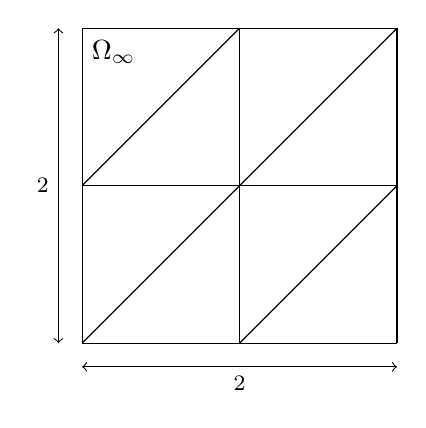
\begin{tikzpicture} [dot/.style={draw,rectangle,minimum size=4mm,inner sep=0pt,outer sep=0pt,thick}, step=2cm]
		\draw [thin] (0,0) grid (4,4);
		\draw [thin] (0,2) -- (2,4);
		\draw [thin] (0,0) -- (4,4);
		\draw [thin] (2,0) -- (4,2);
		\node [font=\normalsize] at (0.4,3.7) {$\Omega_\infty$};
	% \begin{tikzpicture} [dot/.style={draw,rectangle,minimum size=4mm,inner sep=0pt,outer sep=0pt,thick}]
		% \draw [thin] (0,0) grid (4,4);
		% \draw [thin] (0,3) -- (1,4);
		% \draw [thin] (0,2) -- (2,4);
		% \draw [thin] (0,1) -- (3,4);
		% \draw [thin] (0,0) -- (4,4);
		% \draw [thin] (1,0) -- (4,3);
		% \draw [thin] (2,0) -- (4,2);
		% \draw [thin] (3,0) -- (4,1);
		% \node [font=\normalsize] at (0.35,3.75) {$\Omega_\infty$};
		\draw [thin,<->] (0,-0.3) -- (4,-0.3) node[draw=none,fill=none,font=\footnotesize,midway,below] {2};
		\draw [thin,<->] (-0.3,0) -- (-0.3,4) node[draw=none,fill=none,font=\footnotesize,midway,left] {2};
	\end{tikzpicture}
%	\qquad\qquad
%	\begin{tikzpicture}
%		\draw[thin] (2,2) circle (2 cm);
%		\draw[thin] (1.29289321882,1.29289321882) -- (1.29289321882,2.70710678118);
%		\draw[thin] (1.29289321882,1.29289321882) -- (2.70710678118,1.29289321882);
%		\draw[thin] (2.70710678118,2.70710678118) -- (2.70710678118,1.29289321882);
%		\draw[thin] (2.70710678118,2.70710678118) -- (1.29289321882,2.70710678118);
%		\draw[thin] (0.58578643763,0.58578643763) -- (1.29289321882,1.29289321882);
%		\draw[thin] (3.41421356236,3.41421356236) -- (2.70710678118,2.70710678118);
%		\draw[thin] (3.41421356236,0.58578643763) -- (2.70710678118,1.29289321882);
%		\draw[thin] (0.58578643763,3.41421356236) -- (1.29289321882,2.70710678118);
%		% \node at (2,2) {\includegraphics[clip=true, trim = 0.5cm 0 0.5cm 4cm, width=0.4\textwidth]{Figures/Obstacle_mesh.png}};
%		\draw [thin,<->] (0,-0.3) -- (4,-0.3) node[draw=none,fill=none,font=\footnotesize,midway,below] {2};
%		\node [font=\normalsize] at (0.4,3.7) {$\Omega_2$};
%    \end{tikzpicture}
	\caption{\label{fig:ObstacleMesh}
	 Initial FE mesh for domains $\Omega_\infty$
	 %, $\Omega_{2}$ mesh sizes $h = h_\infty, h_2$, respectively.
	 % (l): Initial triangular mesh for $(\mathbb{P}_p\text{-bubble},\mathbb{P}_{p-1}\text{-broken})$ pair on $\Omega_\infty$.
	%(r): Initial quadrilateral mesh for $(\mathbb{Q}_p\text{-bubble},\mathbb{Q}_{p-1}\text{-broken})$ pair on $\Omega_2$.
	 %We consider various polynomial orders $p \geq 1$ and mesh sizes.
	 }
\end{figure}
\end{minipage}    
    % Button to go back
    \hyperlink{example_1}{\beamerbutton{Back to Example 1}}
\end{frame}

\end{document}

\appendix

\section*{Extensions of Proximal Galerkin}
\begin{frame}\frametitle{Nonsymmetric VI}
{\Large
{\color{Maroon}
What about variational inequalities that do not arise as energy minimization principles?
}
}
\end{frame}

\begin{frame}\frametitle{Ext. 1: Discrete Maximum Principle}
\begin{itemize}
\item
Let $\epsilon > 0$, $\beta \in \mathbb{R}^d$ be fixed, $f \in L^\infty(\Omega)$, and $g \in H^1(\Omega) \cap C(\overline{\Omega})$. 
\item The solution $u$ to the advection diffusion equation should satisfy a maximum principle on the continuous and \textbf{discrete} level:
\begin{equation}
\label{eq:AdvectionDiffusionEquation}
	-\epsilon\Delta u + \beta\cdot\nabla u = f
	\quad \text{in~} \Omega,
	\qquad
	u = g \quad \text{on~} \partial\Omega
	\,,
\end{equation}
\item By rewriting \eqref{eq:AdvectionDiffusionEquation} as a variational inequality, we can develop a Proximal Galerkin scheme.
\item There are (many) details in the paper including a ``binary entropic Poisson equation'', an implementable algorithm, further pairs of tailored FE spaces for the new saddle point problems.
\end{itemize}
\end{frame}

\begin{frame}\frametitle{Ext. 1: Discrete Maximum Principle}
\begin{figure}
	\centering
	\begin{minipage}{0.3\textwidth}
	\small
		\centering
		\includegraphics[width=\linewidth]{Figures/advection_diffusion_u_exact.png}
		\\
		Exact solution $u$
	\end{minipage}%,
	\
	\begin{minipage}{0.03\textwidth}
	\small
		\centering
		\includegraphics[width=\linewidth]{Figures/advection_diffusion_colorbar.pdf}
		\\[1.5em]
		~
	\end{minipage}%
	~~~
	\begin{minipage}{0.3\textwidth}
	\small
		\centering
		\includegraphics[width=\linewidth]{Figures/advection_diffusion_u_h.png}
		\\
		FEM solution
	\end{minipage}%,
	~
	\begin{minipage}{0.3\textwidth}
	\small
		\centering
		\includegraphics[width=\linewidth]{Figures/advection_diffusion_utilde.png}
		\\
		Proximal Galerkin solution $\tilde{u}_h$
	\end{minipage}%
	\caption{
	Erikkson--Johnson problem with $\epsilon = 10^{-2}$.
	(l):  Exact solution.
	(c): A first-order Bubnov--Galerkin numerical solution that clearly violates the strong maximum principle $0 \leq u(x) \leq 1$.
	(r): $(\mathbb{Q}_1,\mathbb{Q}_1)$-proximal Galerkin solution $\tilde{u}_h = \sigmoid(\psi_h)$ satisfies the strong maximum principle, by construction.
	% These results were obtained with our MFEM implementation \cite{ZenodoCode}.
%	These results can be reproduced by running the MFEM code \texttt{advection\_diffusion.cpp} available at \cite{ZenodoCode}.
	% using $\rho = 1.0$ and $\alpha_k = 0.01$, $k = 1,2,\ldots$
	\label{fig:EJProblem}}
\end{figure}
\end{frame}

\begin{frame}\frametitle{Nonconvex Problems}
{\Large
{\color{Maroon}
What about nonconvex variational problems?
}
}
\end{frame}

\begin{frame}\frametitle{Ext. 2.: Topology Optimization}
\textbf{Find a material distribution with maximum flexibility and a fixed volume}:
\begin{equation}
\label{eq:elastic_compliance_objective}
    \min_{\rho \in L^{\infty}(\Omega)} \ \
    \left\{
    \,
    \widehat{F}(\mathbf{u},\rho)
    =
    \int_{ \Omega} \mathbf{u}\cdot\mathbf{f} \dd \bm{x}
    \,
    \right\}
    \, ,
\end{equation}
subject to the constraints
\begin{equation}
\label{eq:elastic_compliance_constraints}
\left\{\,\,
\begin{gathered}
    -\mathrm{Div} \left( r(\tilde{\rho})\,\bm{\sigma} \right) = \mathbf{f}
    ~~ \text{in }\Omega
    \quad\text{with}\quad
    \mathbf{u} = 0
    ~~\text{on }\Gamma_0
    \,,
    \quad
    \bm{\sigma} \mathbf{n} = 0
    ~~ \text{on }\partial\Omega \setminus \Gamma_0
    \,,
    \\
    -\epsilon^2\Delta \tilde{\rho} + \tilde{\rho}
	= \rho
	~~ \text{in }\Omega
	\quad\text{with}\quad
	\nabla \tilde{\rho}\cdot \mathbf{n} = 0
	~~ \text{on }\partial\Omega
    \,,
    \\
    \int_\Omega \rho(\bm{x}) \dd\bm{x}
    = \theta |\Omega|
    \,,\quad
    0 \leq \rho
    \leq 1
    \,,\quad
    r(\tilde{\rho})
    = \underline{\rho}+ \tilde{\rho}^3 (1-\underline{\rho})
    \,,
\end{gathered}
\right.
\end{equation}
%\end{subequations}
where $\epsilon > 0$ is a \emph{length scale} and $0 < \theta < 1$ is the desired {volume fraction}, which constrains the amount of the domain $\Omega$ occupied by the design.
\end{frame}

\begin{frame}\frametitle{Ext. 2: Topology Optimization}
\begin{figure}
\centering
	\includegraphics[width=7.5cm]{Figures/Cantilever_mesh.png}
	\caption{
	The design domain $\Omega$ for the cantilever beam problem with corresponding boundary conditions and three-element initial mesh with length $h_0 = 1$.
	\label{fig:ElasticCompliance_mesh}}
\end{figure}
\end{frame}

\begin{frame}\frametitle{Mirror Descent}
\begin{itemize}
\item Like proximal point, but replace the objective with its linearization.
\end{itemize}
{\tiny
\begin{algorithm2e}[H]
\DontPrintSemicolon
	\caption{\label{alg:TopologyOptimization}
	Entropic mirror descent for topology optimization.
	}
	\SetKwInOut{Input}{Input}
	\SetKwInOut{Output}{Output}
	\BlankLine
	\Input{
	Initial latent variable $\rho^0 \in L^\infty(\Omega)$, sequence of step sizes $\alpha_k>0$, increment tolerance $\mathtt{itol.} > 0$, and normalized tolerance $\mathtt{ntol.} > 0$.}
	\Output{Optimized material density $\overline{\rho} = \sigmoid(\psi^k)$.}
	\BlankLine
	Initialize $k = 0$.\;
	\While{$\|\sigmoid(\psi^k) - \sigmoid(\psi^{k-1})\|_{L^1(\Omega)} > \min\{\alpha_k\, \mathtt{ntol.},\mathtt{itol.}\}$}
	% \For{$k = 0,1,2,\ldots$}
	{
		\tcp*[l]{Latent space gradient descent}
		Assign $\psi^{k+1/2} \leftarrow  \psi^{k} - \alpha_{k+1} \nabla F(\sigmoid(\psi^k))$.\;
		\tcp*[l]{Compute Lagrange multiplier}
		Solve for $c \in \mathbb R$ such that $\int_\Omega \sigmoid(\psi^{k+1/2} + c) \dd x = \theta |\Omega|$.\;
		\tcp*[l]{Latent space feasibility correction}
		Assign $\psi^{k+1} \leftarrow  \psi^{k+1/2} + c$.\;
		Assign $k \leftarrow k+1$.\;
	}
\end{algorithm2e}
}
\end{frame}

\begin{frame}\frametitle{Ext. 2: Results}
\begin{figure}
\centering
	\centering
	\begin{minipage}[c]{0.96\textwidth}
		\begin{minipage}[c]{0.32\textwidth}
		\small
			\centering
			\includegraphics[width=\textwidth]{Figures/TopOpt/alpha25/Cantilever0.png}
			\\[3pt]
			$k = 0$
		\end{minipage}
		\begin{minipage}[c]{0.32\textwidth}
		\small
			\centering
			\includegraphics[width=\textwidth]{Figures/TopOpt/alpha25/Cantilever6.png}
			\\[3pt]
			$k = 6$
		\end{minipage}
		\begin{minipage}[c]{0.32\textwidth}
		\small
			\centering
			\includegraphics[width=\textwidth]{Figures/TopOpt/alpha25/Cantilever12.png}
			\\[3pt]
			$k = 12$
		\end{minipage}
		\\[7pt]
		\begin{minipage}[c]{0.32\textwidth}
		\small
			\centering
			\includegraphics[width=\textwidth]{Figures/TopOpt/alpha25/Cantilever18.png}
			\\[3pt]
			$k = 18$
		\end{minipage}
		\begin{minipage}[c]{0.32\textwidth}
		\small
			\centering
			\includegraphics[width=\textwidth]{Figures/TopOpt/alpha25/Cantilever24.png}
			\\[3pt]
			$k = 24$
		\end{minipage}
		\begin{minipage}[c]{0.32\textwidth}
		\small
			\centering
			\includegraphics[width=\textwidth]{Figures/TopOpt/alpha25/Cantilever29.png}
			\\[3pt]
			$k = 29$ (final)
		\end{minipage}
	\end{minipage}
	\begin{minipage}[c]{0.032\textwidth}
		\centering
		\includegraphics[width=\textwidth]{Figures/TopOpt/colorbar/colorbar_bw.pdf}
		\\[4pt]~
	\end{minipage}
	% \begin{minipage}[c]{0.96\textwidth}
	% 	\begin{minipage}[c]{0.32\textwidth}
	% 	\small
	% 		\centering
	% 		\includegraphics[width=\textwidth]{Figures/TopOpt/alpha25/Cantilever0.png}
	% 		\\[3pt]
	% 		$k = 0$
	% 	\end{minipage}
	% 	\begin{minipage}[c]{0.32\textwidth}
	% 	\small
	% 		\centering
	% 		\includegraphics[width=\textwidth]{Figures/TopOpt/alpha25/Cantilever10.png}
	% 		\\[3pt]
	% 		$k = 10$
	% 	\end{minipage}
	% 	\begin{minipage}[c]{0.32\textwidth}
	% 	\small
	% 		\centering
	% 		\includegraphics[width=\textwidth]{Figures/TopOpt/alpha25/Cantilever20.png}
	% 		\\[3pt]
	% 		$k = 20$
	% 	\end{minipage}
	% 	\\[7pt]
	% 	\begin{minipage}[c]{0.32\textwidth}
	% 	\small
	% 		\centering
	% 		\includegraphics[width=\textwidth]{Figures/TopOpt/alpha25/Cantilever30.png}
	% 		\\[3pt]
	% 		$k = 30$
	% 	\end{minipage}
	% 	\begin{minipage}[c]{0.32\textwidth}
	% 	\small
	% 		\centering
	% 		\includegraphics[width=\textwidth]{Figures/TopOpt/alpha25/Cantilever40.png}
	% 		\\[3pt]
	% 		$k = 40$
	% 	\end{minipage}
	% 	\begin{minipage}[c]{0.32\textwidth}
	% 	\small
	% 		\centering
	% 		\includegraphics[width=\textwidth]{Figures/TopOpt/alpha25/Cantilever53.png}
	% 		\\[3pt]
	% 		$k = 53$ (final)
	% 	\end{minipage}
	% \end{minipage}
	% \begin{minipage}[c]{0.032\textwidth}
	% 	\centering
	% 	\includegraphics[width=\textwidth]{Figures/TopOpt/colorbar/colorbar_bw.pdf}
	% 	\\[4pt]~
	% \end{minipage}
	\caption{
	% Cantilever beam.
	Subsequence of material densities $\tilde{\rho}_h^k$ from~\Cref{alg:TopologyOptimization} for selected iterations $k$.
	Results obtained with problem parameters $\epsilon = 2\cdot 10^{-2}$ and $\theta = 0.5$; algorithm parameters $\mathtt{itol.} = 10^{-2}$, $\mathtt{ntol.} = 10^{-5}$, and $\alpha_k = 25k$; and discretization parameters $h = h_0/128$ and $p = 1$.
	\label{fig:ElasticCompliance_sequence}}
\end{figure}
\end{frame}


\begin{frame}\frametitle{Finite Element Spaces I}
\begin{itemize}
\item $\mathcal{T}_h$ shape-regular partition of $\Omega \subset \mathbb{R}^2$.
\item $T \in \mathcal{T}_h$ open connected triangular mesh cells with Lipschitz boundaries $\partial T$.
\item  $\Omega := \bigcup_{T \in \mathcal{T}_h} \overline{T}$.
\item $h = \max_{T\in\mathcal{T}_h} \mathrm{diam}(T)$ is the mesh size.
\item $\mathbb{P}_{p}(T)$  space of polynomials of total order up to and including $p$ on a triangle $T$.
%\item $\mathbb{Q}_{p}(T)$ space of tensor-product polynomials of order up to and including $p$ on a quadrilateral $T$.
\item $\mathbb{X}(T)$ of polynomials over an element $T \in \mathcal{T}_h$.
\item We define ``broken'' polynomials 
\[
\mathbb{X}(\mathcal{T}_h) = \{\varphi \in L^\infty(\Omega) \mid \varphi_{|T} \in \mathbb{X}(T) \text{~for every~} T \in \mathcal{T}_h\}.
\]
\item \pause There is an analogous construction for quadrilaterals in the paper.
\end{itemize}

\end{frame}

\begin{frame}\frametitle{Finite Element Spaces II}
\begin{itemize}
\item We require spaces of degree-$q$ polynomials on whose traces on the cell boundary $\partial T$ have lower polynomial degree $p < q$.
\item Define the sets of bubble functions in $\mathbb{P}_{q}(T)$
 %and $\mathbb{Q}_{q}(T)$ 
 to be 
\[
\aligned
\mathring{\mathbb{P}}^{q}(T) &= \{ \varphi \in \mathbb{P}_{q}(T) \mid \varphi_{|\partial T} =  0\}%\\
%\mathring{\mathbb{Q}}^{q}(T) &= \{ \varphi \in \mathbb{Q}_{q}(T) \mid \varphi_{|\partial T} =  0\}
\endaligned
\]
\item Then define 
\[
\aligned
\hat{\mathbb{P}}_{p}(T) &= \mathbb{P}_{p}(T) \setminus \mathring{\mathbb{P}}^{p}(T)%\\
%\hat{\mathbb{Q}}_{p}(T) &= \mathbb{Q}_{p}(T) \setminus \mathring{\mathbb{Q}}^{p}(T)
\endaligned
\]
\item Finally
let
\begin{equation}
	\mathbb{P}_p^q(T) = \hat{\mathbb{P}}_{p}(T) \oplus \mathring{\mathbb{P}}^{q}(T).
%	\quad
%	\text{and}
%	\quad
%	\mathbb{Q}_p^q(T) = \hat{\mathbb{Q}}_{p}(T) \oplus \mathring{\mathbb{Q}}^{q}(T)
%	\,.
\end{equation}
\end{itemize}
\end{frame}

\begin{frame}\frametitle{Finite Element Spaces III}
For any integer $p \geq 1$, we define the following pairs of spaces:
%\begin{subequations}
\label{eq:SubspacePairs}
\smallskip
%\noindent\textsl{Triangular elements.} 
We refer to the following as the $(\mathbb{P}_p\text{-bubble},\mathbb{P}_{p-1}\text{-broken})$ pairing:
\begin{equation*}
\label{eq:SubspacePair1}
	V_h = \mathbb{P}_{p}^{p+2}(\mathcal{T}_h)\cap H^1_0(\Omega)
	\,,\qquad
	% \quad
	% \text{and}
	% \quad
	W_h = \mathbb{P}_{p-1}(\mathcal{T}_h)
	\,.
\end{equation*}
% \medskip
%
%\noindent\textsl{Quadrilateral elements.} We refer to the following as the $(\mathbb{Q}_p\text{-bubble},\mathbb{Q}_{p-1}\text{-broken})$ pairing:
%\begin{equation}
%\label{eq:SubspacePair2}
%	V_h = \mathbb{Q}_{p}^{p+1}(\mathcal{T}_h)\cap H^1_0(\Omega)
%	\,,\qquad
%	% \quad
%	% % V_h = \mathbb{Q}_{p+2}(\mathcal{T}_h)\cap H^1_0(\Omega)
%	% \quad
%	% \text{and}
%	% \quad
%	W_h = \mathbb{Q}_{p-1}(\mathcal{T}_h)
%	\,.
%\end{equation}
%\end{subequations}
\vspace{-3ex}
\begin{itemize}
\item Example, $p = 1$: $V_h$ is composed of the direct sum of piecewise linear functions and 3rd order bubble functions and $W_h$ is piecewise constants. \pause
\item
For shape regular $\mathcal{T}_h$, these pairs of spaces are \textbf{stable} for the linearized, singularly perturbed saddle point problems.
\item 
The paper contains similar spaces for quadrilateral mesh cells and alternative pairs without bubble functions that are also stable.
\end{itemize}
\end{frame}
\end{document}

# degrees of freedom: 121 (25, 96)
   0 SNES Function norm 1.059989593778e+01
   1 SNES Function norm 1.877676778142e+00
   2 SNES Function norm 2.712593468704e-01
   3 SNES Function norm 9.785071866286e-03
   4 SNES Function norm 1.488837921188e-05
   5 SNES Function norm 4.370623027203e-11
# degrees of freedom: 433 (81, 352)
   0 SNES Function norm 3.013033401065e+01
   1 SNES Function norm 4.930874839744e+00
   2 SNES Function norm 1.156998579063e+00
   3 SNES Function norm 1.478952300402e-01
   4 SNES Function norm 3.950686295158e-03
   5 SNES Function norm 3.473244156342e-06
   6 SNES Function norm 3.534679334821e-12
# degrees of freedom: 1633 (289, 1344)
   0 SNES Function norm 8.714674556331e+01
   1 SNES Function norm 8.794270828755e+00
   2 SNES Function norm 2.608988329166e+00
   3 SNES Function norm 6.123840123053e-01
   4 SNES Function norm 7.470097718825e-02
   5 SNES Function norm 1.715331436107e-03
   6 SNES Function norm 1.137083665986e-06
   7 SNES Function norm 6.970740750155e-13
# degrees of freedom: 6337 (1089, 5248)
   0 SNES Function norm 2.494585793077e+02
   1 SNES Function norm 1.231111015171e+01
   2 SNES Function norm 4.020536156657e+00
   3 SNES Function norm 1.188639227654e+00
   4 SNES Function norm 2.700114130114e-01
   5 SNES Function norm 2.885432882381e-02
   6 SNES Function norm 4.868112508463e-04
   7 SNES Function norm 1.800505939824e-07
# degrees of freedom: 24961 (4225, 20736)
   0 SNES Function norm 7.089227722247e+02
   1 SNES Function norm 1.528540951662e+01
   2 SNES Function norm 5.220647543972e+00
   3 SNES Function norm 1.689647970872e+00
   4 SNES Function norm 4.886125182388e-01
   5 SNES Function norm 1.030582603411e-01
   6 SNES Function norm 8.812381729669e-03
   7 SNES Function norm 9.209865283391e-05
   8 SNES Function norm 1.355553159695e-08
Errors:  [0.11743707316059077, 0.021397971641314243, 0.0032862218773048496, 0.0005800177797029322, 0.00012470641099309474]
Convergence orders:  [2.45634197 2.70297225 2.50226086 2.21756149]



